\chapter{细胞和组织的适应、损伤}

\chapterabstract{本章主要介绍组织细胞在病理因素刺激下所出现的适应性改变、变性、异常物质沉积、坏死、凋亡和损伤机制等内容。要求掌握细胞水肿、脂变及透明变性的形态学特征及其对机体的影响,坏死的形态变化和后果,以及各型坏死的形态学及鉴别点;熟悉各种类型萎缩的形态变化及其对机体的影响,凋亡的概念以及与坏死的鉴别;了解各种色素沉着的形态学特征以及组织细胞损伤的机制。}

正常细胞和组织不断受到内外因子的刺激,其物质代谢、形态结构和功能会因此出现相应改变。若刺激在细胞能承受的有限范围内,则表现为适应,属轻度损伤。若刺激时间长强度大,细胞将发生连续反应,表现为适应、损伤,最终导致细胞死亡。严重损伤可以直接导致细胞死亡。正常细胞、适应细胞、损伤细胞和死亡细胞,这四种状态之间界限不清,在形态结构和代谢、功能上的变化是连续的。活体内细胞死亡发生后,机体将给予修复,最大限度地恢复原有细胞和组织的形态结构和功能。

\section{细胞和组织的适应}

在环境发生变化时,机体的细胞和由其构成的组织、器官为了避免损伤,可通过改变自身的代谢、功能和形态结构以适应变化的环境,这种与之协调的过程称为适应。例如当机体突然进入寒冷环境时会全身发抖,这是对环境适应的表现。“发抖”使肌肉活动加强,糖代谢加速,产热增多,以补偿体表丧失的热量。在病理情况下,如高血压病,左心室心肌纤维肥大,收缩力增强,以克服增高的外周阻力,维持血循环正常进行。这些皆属适应性反应。通过适应反应,机体能维持正常的功能,因此适应是正常细胞和损伤细胞的中间状态,在形态学上的改变表现为萎缩、肥大、增生和化生。

\subsection{萎缩}

发育正常的实质细胞、组织或器官体积缩小称为萎缩(atrophy)。通常是由于该器官的实质细胞体积缩小所致,有时也可因细胞数目减少引起,或二者兼有。萎缩有生理性和病理性之分。生理性萎缩与年龄有关,例如青春期胸腺组织萎缩,妇女绝经后卵巢、子宫、乳腺组织萎缩等属于生理性萎缩。病理性萎缩有的表现为全身性,有的表现为局部组织器官萎缩。

\subsubsection{类型}

常见的病理性萎缩按其发生原因分为以下几种类型:

\paragraph{营养不良性萎缩}
有全身性和局部性两种。消化道慢性梗阻(食管癌)和慢性消耗性疾病(如结核病、晚期癌症患者)引起全身性萎缩。这种萎缩首先发生于对生命不太重要的脂肪组织,其次为肌肉、脾、肝、肾等器官,心、脑等生命重要器官萎缩发生最晚,这样的顺序有一定的代偿适应意义。局部营养不良性萎缩见于局部缺血,如动脉粥样硬化使管壁增厚、管腔狭窄、血流减少,引起心、脑、肾等相应器官萎缩。

\paragraph{压迫性萎缩}
常见于尿路结石,阻塞输尿管,引起尿潴留,不断增加的尿液压迫肾组织,使肾实质逐渐萎缩、变薄,最后,整个肾变为充满液体的薄壁巨囊。
这种萎缩除了压迫的直接作用外,还与压迫引起局部血供不良、废用等因素有关。

\paragraph{废用性萎缩}
亦称失用性萎缩。肢体、器官、组织长期不活动,或只担负轻微的活动,功能减退所引起的萎缩。如骨折后肢体长期固定,肌肉、骨组织萎缩。
这种萎缩的发生还与器官停止活动后,向心性或离心性神经刺激减少或消失有关,以致局部血循环和物质代谢降低。

\paragraph{去神经性萎缩}
因运动神经元或轴突损害导致正常神经调节功能丧失,引起效应组织器官营养障碍或血液循环调节异常,并伴有组织功能减低或丧失等综合因素,导致相应部位萎缩。
例如小儿麻痹症(脊髓前角灰质炎)患者由于脊髓前角运动神经细胞死亡,结果受这些细胞支配的肢体肌肉发生麻痹,逐渐萎缩,同时患肢骨小梁变细,钙盐减少,骨质疏松,肢体变得细短。

\paragraph{内分泌性萎缩}
内分泌功能低下时,它所作用的靶器官发生萎缩。如席蒙病(Simmond's
disease)时,由于垂体受到损伤,各种促激素分泌减少,常引起甲状腺、肾上腺、性腺等靶器官萎缩。
老年性萎缩虽然是一种生理现象,也属老年病。
发生机制复杂,与老年期内分泌功能低下、血管硬化、供血不良及运动量减少等众多因素有关。
临床上,某种萎缩可由多种因素所致。

\subsubsection{病理形态}

肉眼观:萎缩的细胞、组织、器官体积变小,重量减轻,颜色变深常呈褐色。
心肌萎缩时冠状动脉在心外膜下呈蛇行弯曲(图\ref{fig1-1}a)。
脑萎缩时,脑回变窄,脑沟变深加宽。镜下观:萎缩的细胞体积变小,或数目减少或两者兼有。
胞浆常深染,核浓缩。心肌萎缩时,其胞浆内可出现棕褐色颗粒,即脂褐素(图\ref{fig1-1}b)。
\begin{figure}[!htbp]
	\centering
	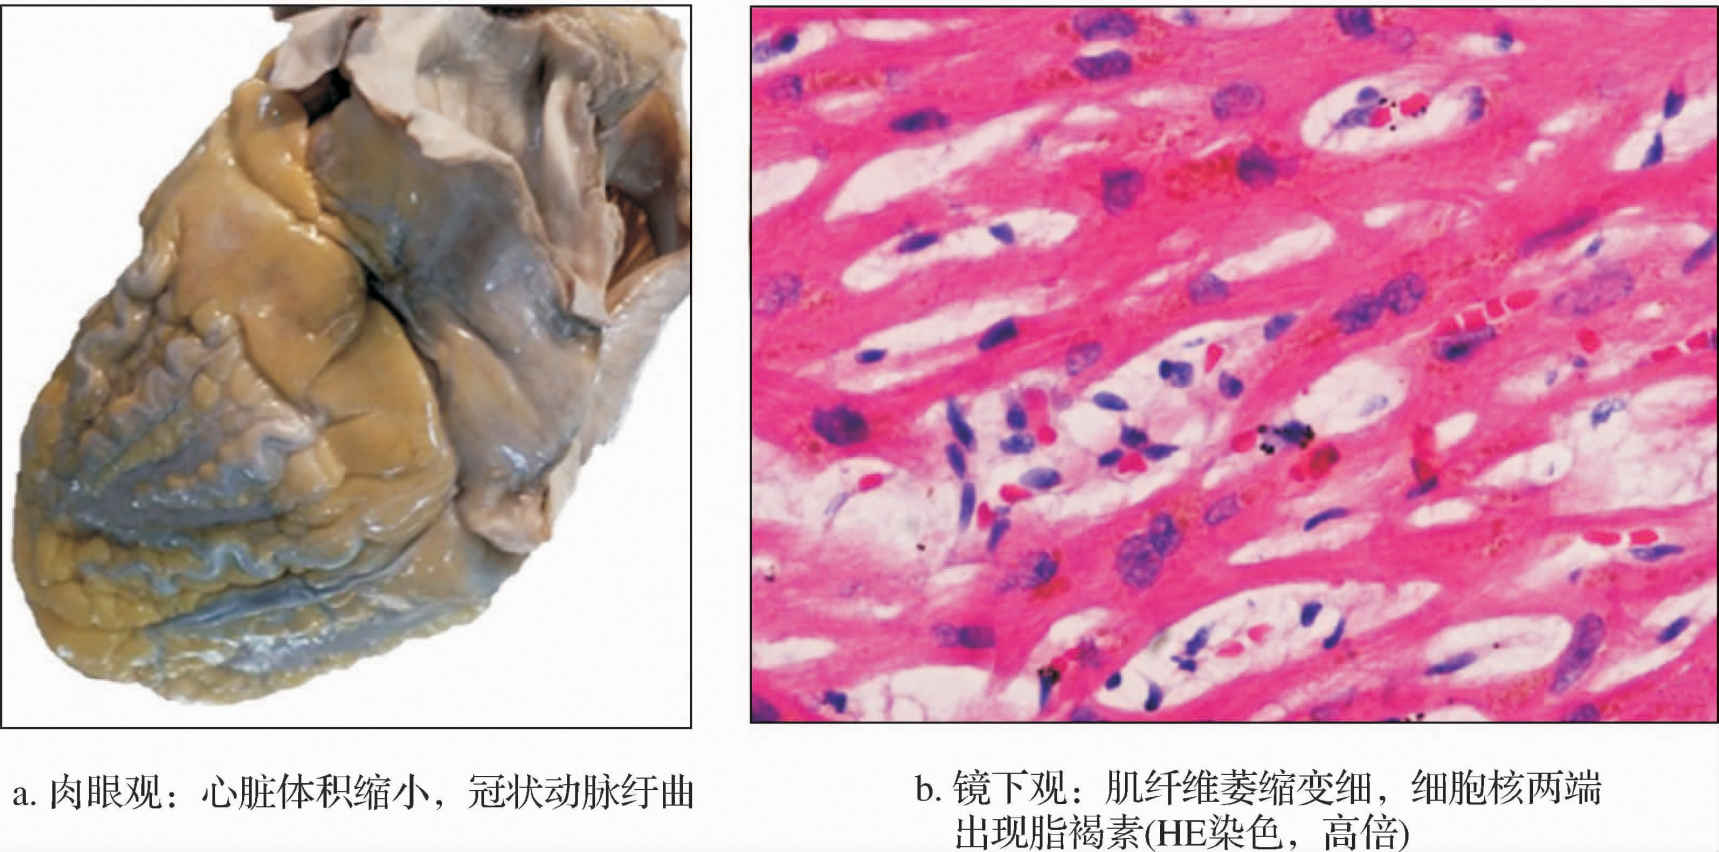
\includegraphics[width=.8\textwidth]{./images/Image00002.jpg}
	\caption{心肌萎缩}
	\label{fig1-1}
\end{figure}
%\FloatBarrier

萎缩的机制尚未完全搞清,蛋白合成少于分解可能为主要原因。

萎缩的器官、组织、细胞功能常降低,但一般是可复性的。原因消除后,萎缩的器官也可恢复正常。如原因持续存在,萎缩的实质细胞最后消失,间质结缔组织和脂肪细胞可以增生,甚至造成器官和组织体积增大,此时称假性肥大。

\subsection{肥大}

由于功能增加、合成代谢旺盛,细胞体积增大,使该器官、组织体积增大,称为肥大(hypertrophy)。肥大多发生于无分裂增殖能力或增殖能力较弱的细胞,如心肌、骨骼肌等。一般可分为生理性肥大和病理性肥大两类。如举重运动员上臂和胸部肌肉的粗壮肥大,妊娠子宫平滑肌细胞肥大属生理性肥大。病理情况下,也可发生肥大。例如高血压病,左心功能负荷加重,心肌纤维体积增大,一侧肾切除后另一侧肾体积增大,皆属代偿性肥大。而成人脑垂体前叶嗜酸细胞瘤分泌过多生长激素,导致的肢端肥大症,则属内分泌性肥大。肥大的细胞除了体积增大外,其内细胞器和微丝明显增多,蛋白合成旺盛。

有时实质细胞萎缩,间质增生也可使该器官、组织体积增大,这种假性肥大与前述的真性肥大有本质的区别。

\subsection{增生}

实质细胞数量增多,使该组织、器官体积增大,称为增生(hyperplasia)。增生可分为生理性和病理性增生两类。妇女在青春期、妊娠期和哺乳期乳腺上皮增生属生理性增生。病理情况下,例如溶血性贫血时骨髓的红细胞系增生,长期缺碘引起甲状腺组织增生,慢性鼻炎黏膜增生肥厚形成息肉等属于病理性增生。由于引起细胞、组织和器官增生与肥大的原因往往十分相似或相同,故两者常同时出现。这种现象见于雌激素过多时引起的子宫内膜增生、乳腺增生,以及老年男性因雄激素代谢障碍导致的前列腺增生。

\subsection{化生}

化生(metaplasia)是指一种已分化成熟的细胞由于适应环境改变而被另一种分化成熟细胞所代替的过程。化生并不是由一种成熟的细胞直接转变为另一种成熟的细胞,而是由该处具有分裂增殖和多向分化能力的幼稚细胞增生,向另一种类型的细胞分化、成熟,也就是所谓的异向分化,是环境因素引起细胞某些基因活化或受到抑制而重新编程表达的结果。化生常发生于同源细胞间,如一种上皮细胞与另一种上皮细胞间。化生是一种可复性病变,原因去除后大多可恢复。常见的化生有:

\subsubsection{鳞状上皮化生}

慢性支气管炎或长期吸烟者,气管及支气管的纤毛上皮转变为鳞状上皮。慢性胆囊炎及胆石症时,胆囊黏膜上皮发生鳞状上皮化生。慢性宫颈炎、子宫内膜炎时,黏膜上皮发生鳞状化生,在妇产科极为常见(图\ref{fig1-2})。肾盂结石时,肾盂黏膜的移行上皮也可转变为鳞状上皮。
\begin{figure}[!htbp]
	\centering
	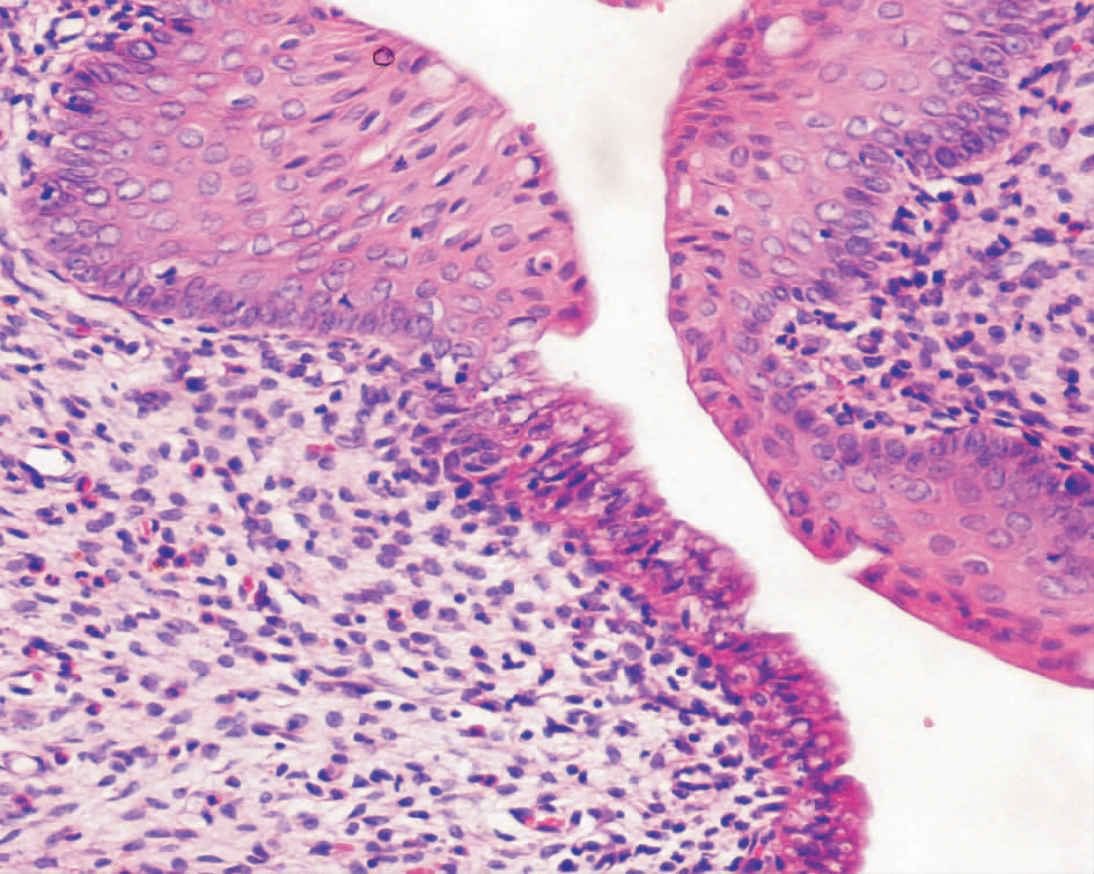
\includegraphics{./images/Image00003.jpg}
	\caption{子宫内膜鳞状上皮化生(HE染色,高倍) \\ {\small 子宫内膜的纤毛柱状上皮化生为鳞状上皮}}
	\label{fig1-2}
\end{figure}
%\FloatBarrier

\begin{framed}
	{案例1-1}

	{【病例摘要】}

	患者,男,55岁,因醉酒后呕吐、误吸,呛咳、呼吸困难入院。全麻下行支气管镜检查,从右主支气管中取出少量未消化米粒和菜叶,症状缓解;术中发现支气管黏膜充血、粗糙,征得家属同意后,夹取2块黏膜组织送病理检查。患者有吸烟史30年,反复咳嗽、咳痰史10年,否认其他病史。病理报告为“送检组织为少量鳞状上皮及其下疏松结缔组织、腺体,伴小血管充血和淋巴细胞、浆细胞浸润。符合慢性支气管炎。”

	{【问题】}

	(1)该患者支气管黏膜出现鳞状上皮,此属何种病理现象?

	(2)试分析病变形成机制和意义。
\end{framed}

\subsubsection{肠上皮化生}

慢性胃炎时,部分胃黏膜上皮转变为含有杯状细胞、潘氏细胞及具有纹状缘的吸收上皮,与小肠黏膜上皮相似;或在柱状上皮中,间有杯状细胞,与大肠黏膜上皮相似,均称为肠上皮化生(简称肠化)。类似的化生也常发生于腺体,由一种腺上皮转变为另一种腺上皮,故又称腺性化生。

\subsubsection{结缔组织和支持组织化生}

纤维组织化生为脂肪组织或肌细胞,成纤维细胞转变为骨母细胞或软骨母细胞,分别化生为骨或软骨(图\ref{fig1-3})。
\begin{figure}[!htbp]
	\centering
	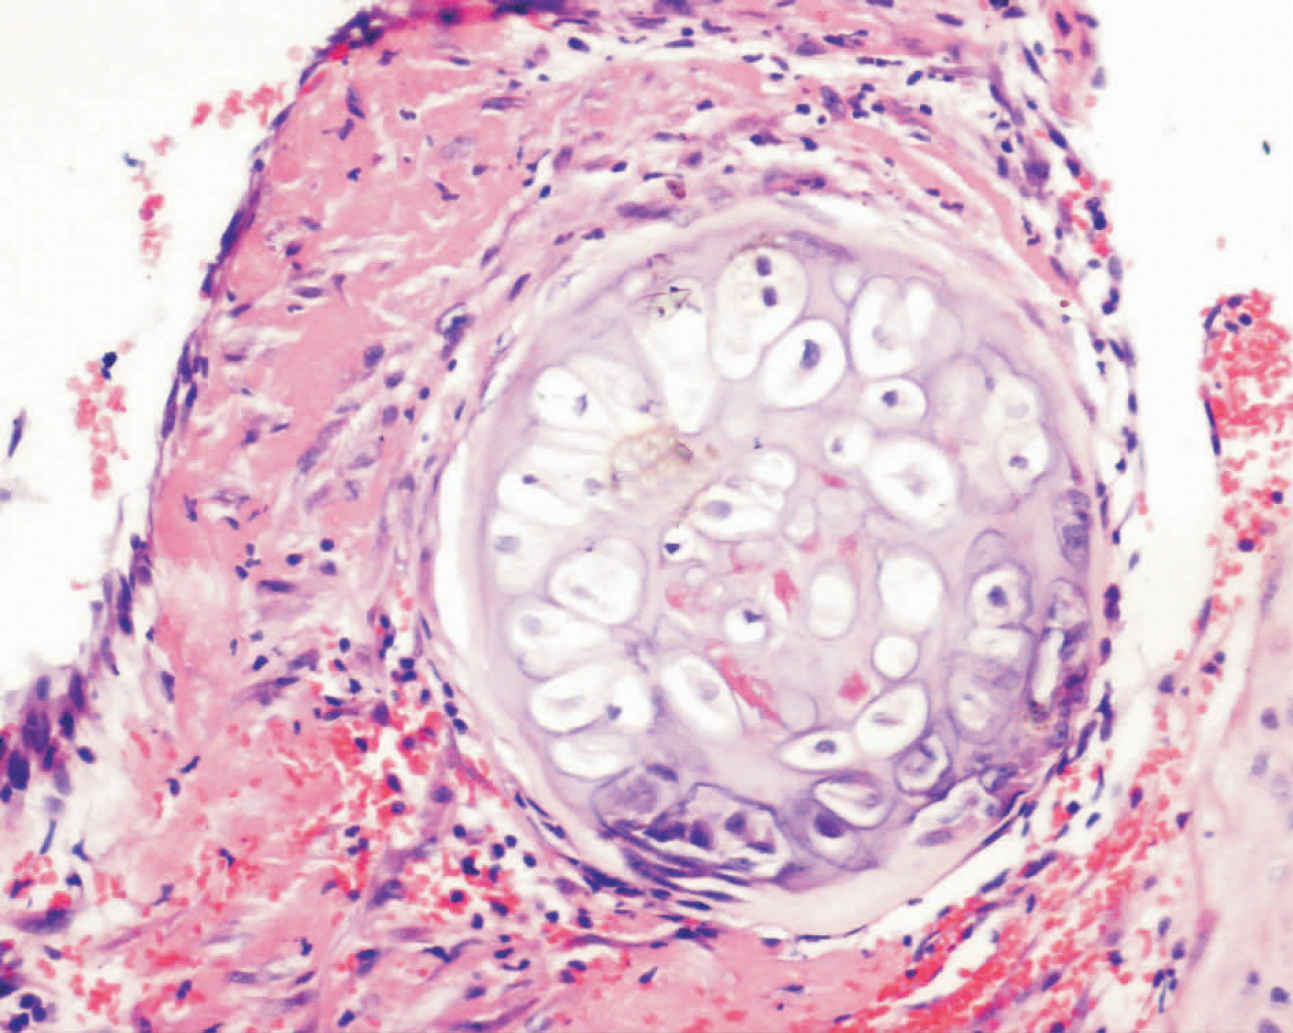
\includegraphics{./images/Image00004.jpg}
	\caption{心瓣膜软骨化生(HE染色,高倍) \\ {\small 心瓣膜结缔组织出现软骨化生}}
	\label{fig1-3}
\end{figure}
%\FloatBarrier

\begin{center}
	\textbf{知识链接}
\end{center}
\chapterabstract{上皮间质转分化(epithelial-mesenchymal
transition)为近年研究热点,其实也是一种化生现象。它是指上皮细胞在某些因素刺激下,逐渐失去上皮细胞表型(如E钙黏蛋白、细胞骨架蛋白等的表达)而呈现间质细胞表型(如波形蛋白、平滑肌肌动蛋白、纤维连接蛋白等的表达)。该现象可见于多种生理病理过程,如胚胎发育、组织重塑、肿瘤侵袭转移、慢性炎症和器官纤维化等。}

化生是机体对环境中不良因子发生防御反应的一种形式,对机体是有利的,但也有其局限性和不完善性。例如支气管黏膜鳞状化生后,失去纤毛,削弱了黏膜的自净能力。在化生、增生的基础上,还可能发展为肿瘤。例如支气管鳞状上皮化生和胃黏膜肠上皮化生,分别与肺鳞状细胞癌和胃腺癌的发生有一定的关系。

综上所述,组织细胞为了适应内外环境的变化,可出现萎缩、肥大、增生和化生等形态学改变(图\ref{fig1-4})。若刺激因素使发育正常的组织或器官内实质细胞体积缩小或数目减少即称为萎缩;实质细胞体积增大,即称为肥大;实质细胞数量增多,即称为增生;已分化成熟的细胞被另一种分化成熟细胞所代替即称为化生。

\begin{figure}[!htbp]
	\centering
	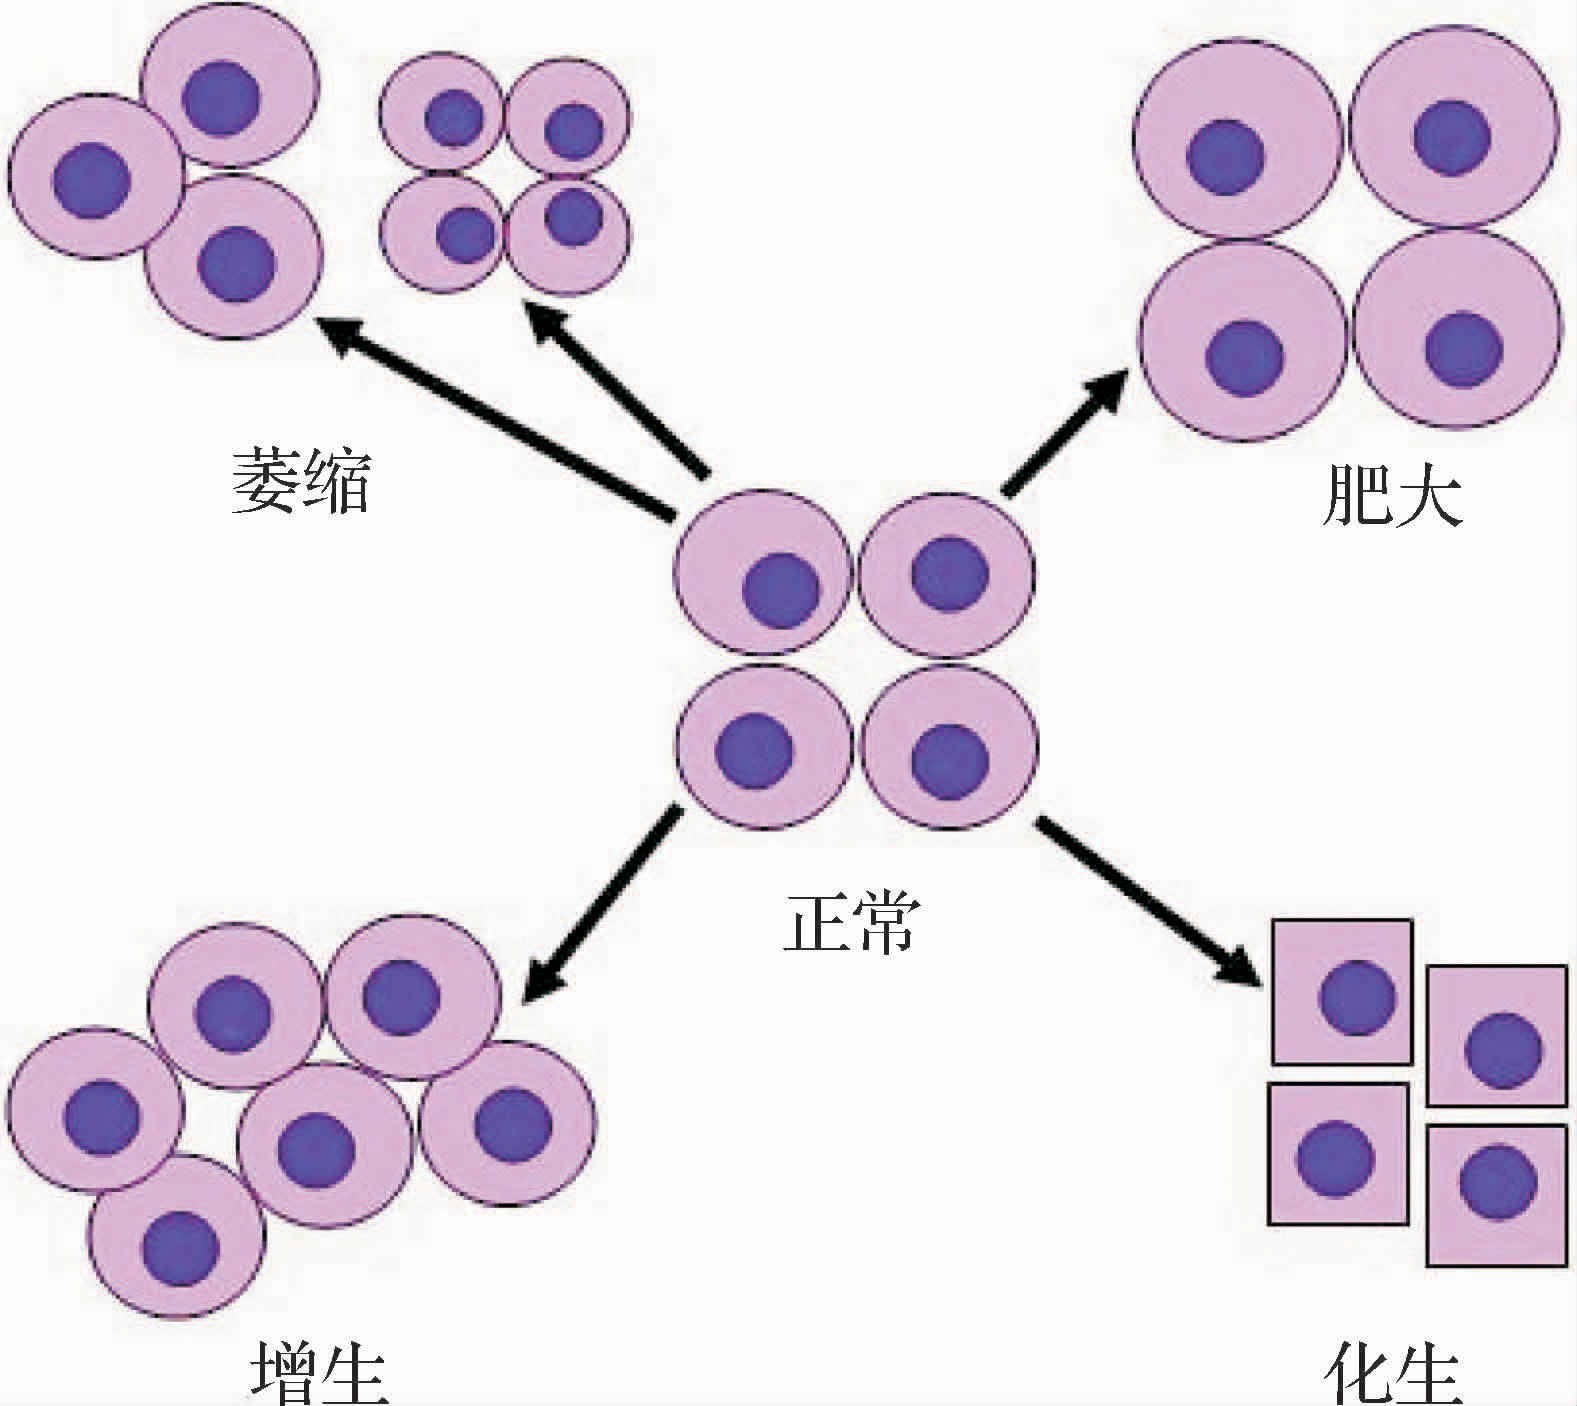
\includegraphics{./images/Image00005.jpg}
	\caption{四种适应性改变示意图}
	\label{fig1-4}
\end{figure}
%\FloatBarrier

\section{细胞和组织的损伤}

当损伤因素超出机体的适应能力,则引起细胞和组织的损伤。在一定程度内这种损伤为可复性,形态上表现为变性和物质异常沉积。重度损伤则引起细胞和组织的死亡。

\subsection{细胞和组织损伤的原因与发生机制}

\subsubsection{缺氧}

缺氧是引起组织细胞损伤常见而重要的原因。缺氧常见于:各种原因造成动脉供血不足或静脉回流障碍,或由于呼吸、循环障碍使血氧含量不足,也可见于严重贫血或中毒(如CO中毒)使红细胞携氧能力降低等情况。缺氧首先影响细胞的需氧呼吸,即线粒体的氧化磷酸化功能,使ATP产生减少或停止,导致细胞膜的钠泵功能障碍,Na{+}
及水在细胞内集聚,K{+}
从细胞外溢,造成急性细胞肿胀。缺氧也使无氧酵解过程增强,通过糖原分解产生ATP,以维持细胞的能量,但在无氧酵解的过程中细胞内乳酸、酮体、氨基酸和无机酸等氧化不全的代谢产物大量积聚,使pH下降。随之粗面内质网核蛋白体脱失、裂解,并出现线粒体肿胀,内质网扩张等一系列超微结构改变。以上改变是可复性的,随缺氧的恢复而恢复正常。如缺氧持续存在,ATP供应耗竭,细胞酶系统广泛损伤,细胞膜功能严重受损,细胞外Ca{2+}
不断进入细胞内,甚至进入线粒体内,使其基质中出现无定形的富于钙的致密区,线粒体发生不可复性改变,以至参与代谢的某些酶活性受抑,并使蛋白变性,细胞死亡。细胞内pH进一步下降将导致溶酶体膜的损伤,其内多种酶进入细胞浆内并被激活,其中酸性水解酶可引起细胞自溶死亡。

不同组织细胞对缺氧的耐受程度不同。结缔组织对缺氧耐受时间最长,而神经细胞对氧极为敏感,缺氧长于5~10分钟,细胞则发生不可复性损伤。

\subsubsection{物理因子}

物理因子包括机械性、高温、低温、电流、放射线等刺激因子。机械性损伤能使细胞组织破裂;高温使细胞内蛋白质(包括酶)变性,低温可使血管收缩引起组织缺血性损伤,或造成局部血流停滞、凝血,甚至细胞内水分形成冰晶而损伤细胞;电流通过组织时引起高温灼伤局部组织;放射线作用于机体能直接或间接造成大分子损伤,使水分被激发电离,产生大量具有强毒力的自由基,损伤组织细胞。物理因子引起损伤的严重程度主要决定于该物理因子的作用性质、强度和持续时间的长短,而很少和机体的反应性有关。

\subsubsection{化学因子}

许多化学物质进入人体,在组织细胞内发生化学反应,可破坏正常的生理功能。化学物质造成组织损伤前提是它们必须能经口、呼吸道、皮肤或黏膜进入体内才能引起中毒。化学因子引起损伤的机制是多方面的:①直接损伤:如强酸、强碱可直接灼伤皮肤或黏膜,引起局部炎症或坏死;②抑制酶的活性:如有机磷农药能抑制胆碱酯酶的活性,引起损伤。氯化汞和体内的巯基结合,从而使许多酶蛋白失去活性或破坏膜蛋白结构;③通过代谢形成毒性代谢产物而发挥作用:例如,四氯化碳经肝细胞滑面内质网所含的细胞色素P-450混合功能氧化酶类的作用,裂解生成毒性物质CCl{3}
和Cl自由基,后者可引起肝细胞发生脂肪变性和坏死。

自由基(free
radical)又称游离基,是指一类含有未配对电子的化学基团,如H{+} 、OH{-}
、HOO、O{2-}
,其化学活性高而不稳定,它与细胞内各种有机或无机化合物,如脂质、蛋白质、核酸等,发生过氧化、交联或断裂,从而造成细胞的损伤。但在正常人体内,自由基在细胞外液中的浓度极低,不构成对细胞的威胁,而在吞噬细胞杀灭病原生物或抗肿瘤细胞过程中自由基却起重要防御作用。但是如果体内生成过多,或清除障碍,如在上述的化学性、放射性、炎症损伤过程中,或随着年龄的增长,机体抗氧化活性递减,逐级降低对自由基的防御能力,均可引起组织细胞损伤或机体衰老。自由基可在正常新陈代谢中产生,是普遍存在于生物系统的代谢中间产物,种类多,数量大,活性高。

\subsubsection{生物性因子}

生物性因子是引起细胞损伤最常见的原因,包括病毒、细菌、立克氏体、真菌、寄生虫等引起的各种感染。其作用机制有下列几方面:①直接作用损伤细胞和组织:病毒寄生于细胞内干扰细胞的代谢活动,使细胞变性坏死。②通过内外毒素的作用或产生的毒性代谢产物:如白喉外毒素自由基能抑制细胞的氧化过程和蛋白质的合成。溶血性链球菌产生的透明质酸酶和链激酶引起间质损伤。③生物因子具有抗原性,能引起变态反应:肝炎病毒有嗜肝细胞的特性并产生病毒蛋白,后者可通过变态反应引起肝细胞损伤。

\subsubsection{免疫反应}

免疫反应是机体的正常防御功能,通过免疫反应排斥异己物质,以维持内环境的稳定。但这种反应结果并非均对机体有利,例如病毒性肝炎,在机体T细胞致敏清除肝炎病毒的过程中也造成肝细胞的损伤;在某些情况下对病原生物产生的抗体与体内组织抗原发生交叉反应,形成抗原抗体复合物沉积于组织,引起损伤,如风湿性心肌炎,急性肾小球肾炎,通过变态反应对自身组织抗原发生反应,引起组织细胞的损伤;甚至针对自身组织发生自身免疫反应,如红斑性狼疮,类风湿关节炎等。

\subsubsection{其他}

遗传缺陷、营养失衡、内分泌异常、衰老、心理和社会因素等也能导致组织细胞的损伤。

综上所述,引起组织细胞损伤的因子很多,它们主要通过以下几个途径造成细胞损伤(图\ref{fig1-5}):①ATP耗竭,细胞需要能量的生理活动受阻;②细胞膜完整性破坏、渗透性缺陷,导致细胞内容物流失或物质交换和电生理活动异常;③细胞内钙离子浓度升高,多种酶被激活,使ATP耗竭或细胞结构的破坏;④自由基产生增多;⑤其他代谢活动异常等。一种因子可通过多种途径损伤细胞,几种因子亦可共用一条途径使细胞受累。
\begin{figure}[!htbp]
	\centering
	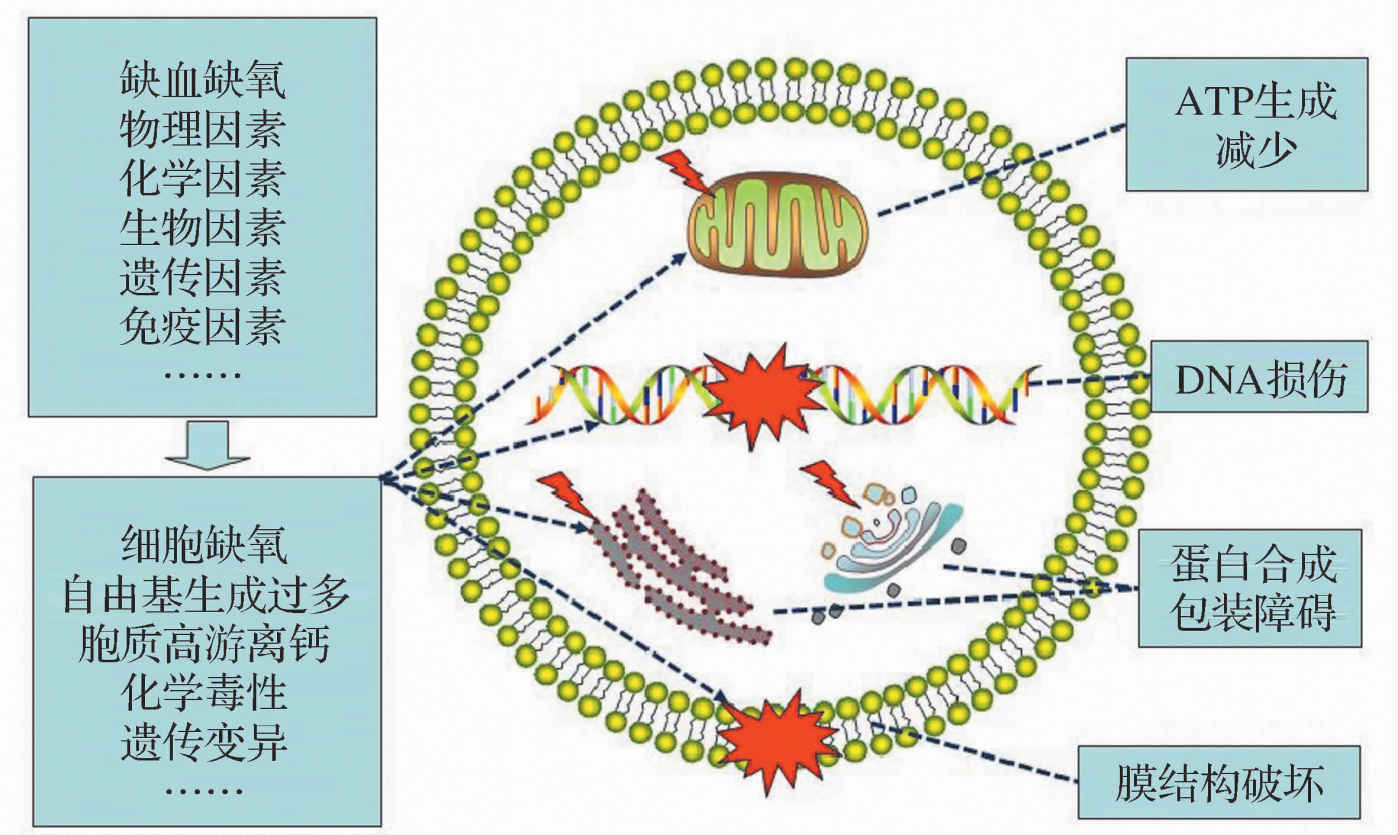
\includegraphics{./images/Image00006.jpg}
	\caption{组织细胞损伤机制示意图}
	\label{fig1-5}
\end{figure}
%\FloatBarrier 

\subsection{细胞和组织损伤的形态学变化}

组织细胞损伤有轻重之别,损伤因子强度弱、作用时间短,细胞的损伤可恢复,即为可逆性损伤;若损伤因子持续刺激和过于剧烈,细胞将会死亡,则表现为不可逆性损伤。

\subsubsection{可逆性损伤}

可逆性损伤(reversible
injury),旧称变性(degeneration),是指新陈代谢障碍时,细胞或细胞间质内出现一些异常物质或正常物质异常蓄积。变性的组织细胞功能下降,但通常为可复性,严重者可发展为坏死。变性的种类繁多,下面介绍比较常见的几种变性。

\paragraph{细胞水肿}
细胞水肿(cellular edema)或称水变性(hydropic
degeneration)即细胞内水钠积聚过多,引起细胞体积肿大,胞浆疏松、透明淡染。常见于缺氧、感染、中毒时的心、肝、肾等脏器的实质细胞。

病理上,轻度的细胞水肿,胞浆内出现许多细小的伊红染颗粒,此乃水肿时肿大的线粒体和扩张的内质网,这种变化致相应器官肉眼观时体积轻度增大,包膜紧张,颜色较正常淡,显得混浊而无光泽,在电镜技术问世之前称之为颗粒变性(granular
degeneration)或混浊肿胀,此名词现已弃用。随细胞内水钠积聚增多,细胞水肿进一步发展,线粒体和内质网高度扩张,囊泡变,此时镜下观:胞浆透明、空泡状,故又有空泡变性或水样变性之称(图\ref{fig1-6})。病毒性肝炎和四氯化碳中毒时,肝细胞水肿,严重者细胞肿大如圆球状,特称为气球样变(图\ref{fig1-7})。
\begin{figure}[!htbp]
	\centering
	\begin{minipage}[b]{0.45\textwidth}
		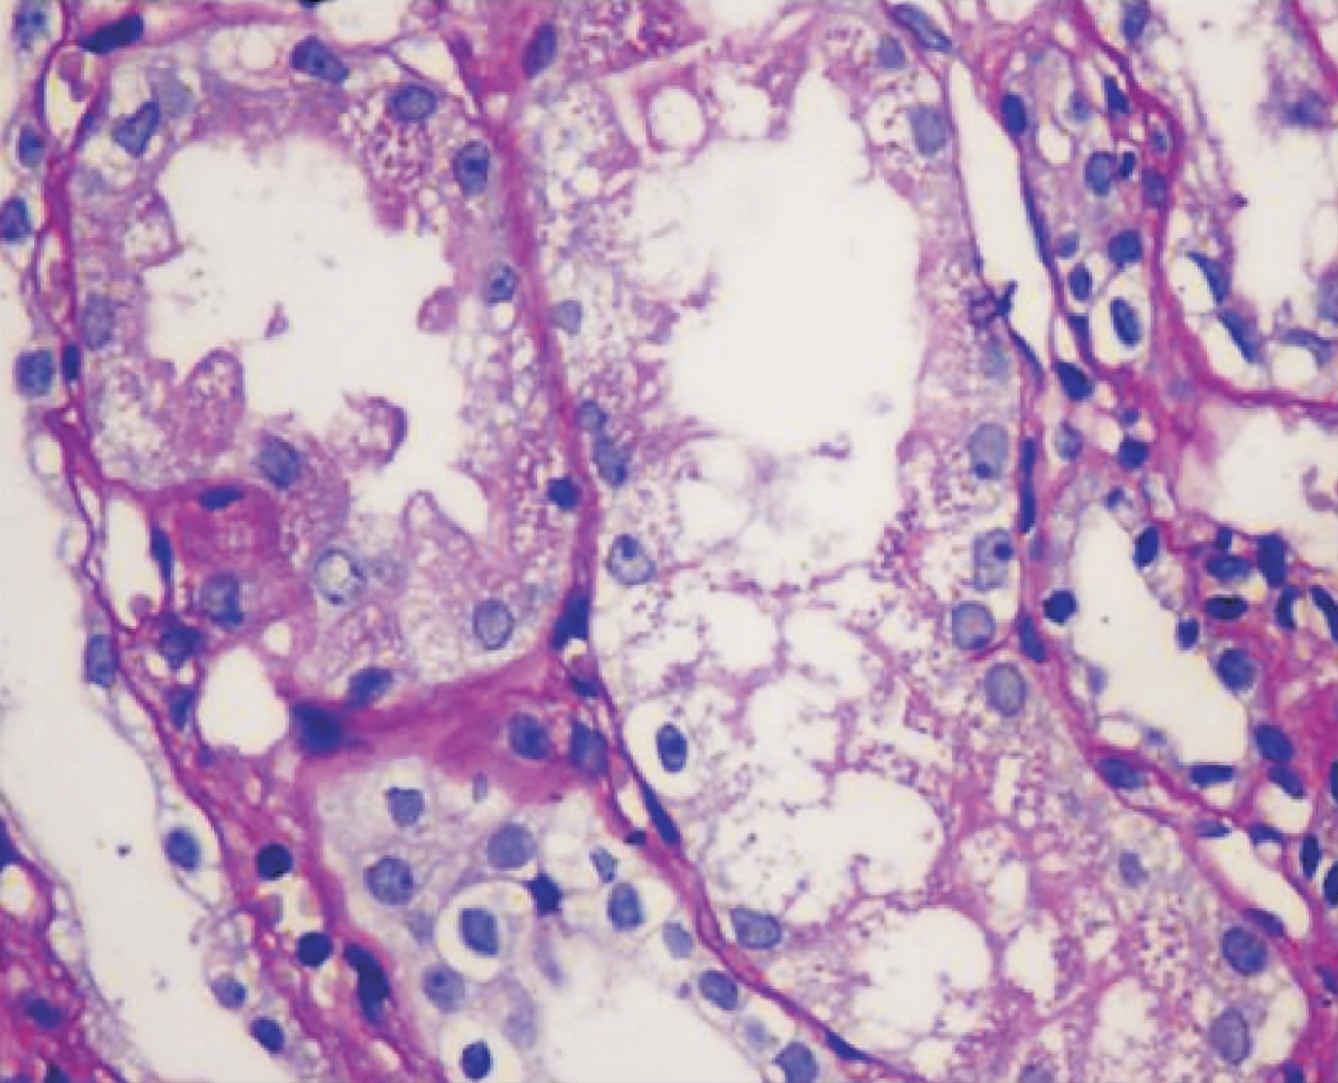
\includegraphics{./images/Image00007.jpg}
		\caption{肾小管上皮细胞水肿(HE染色,高倍) \\ {\small 细胞体积增大,胞浆内出现红染的颗粒状物}}
		\label{fig1-6}
	\end{minipage}
	%	\end{figure} 
	%\FloatBarrier
	%\begin{figure}[!htbp]
	%    \centering
	\hspace{0.04\textwidth}%
	\begin{minipage}[b]{0.45\textwidth}
		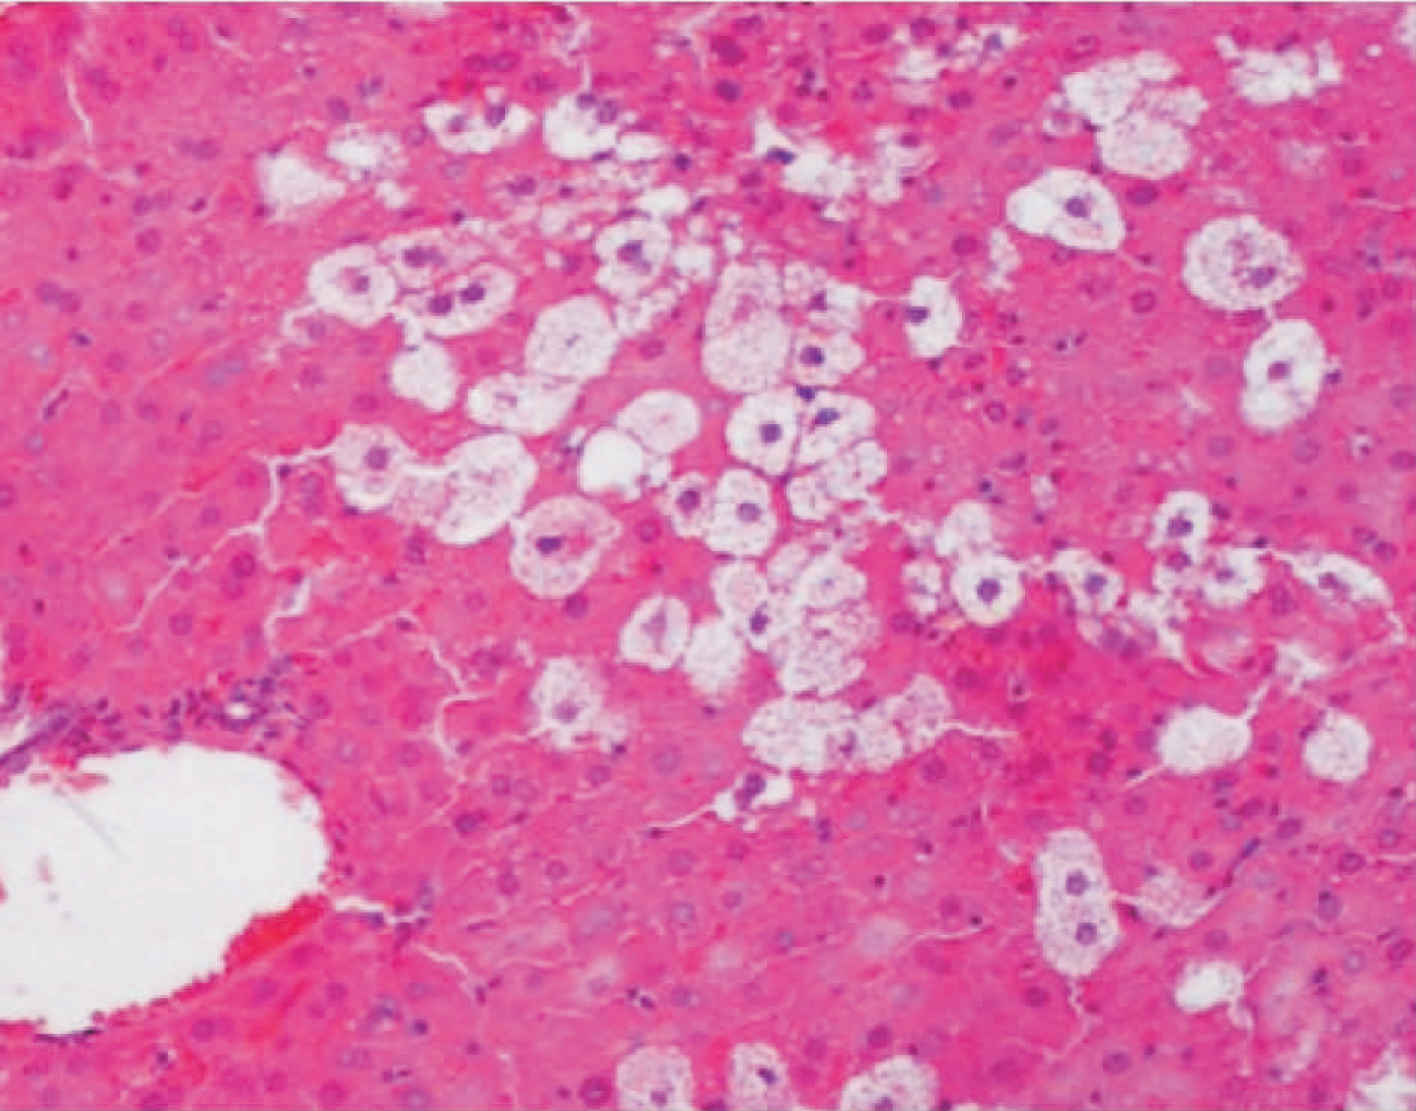
\includegraphics{./images/Image00008.jpg}
		\caption{肝细胞水肿(HE染色,中倍) \\ {\small 肝细胞明显肿胀,细胞浆疏松}}
		\label{fig1-7}
	\end{minipage}
\end{figure}
%\FloatBarrier

引起细胞水肿的原因很多,在急性感染、缺氧、中毒等有害因素的作用下,线粒体产能机制受损,ATP生成减少,使细胞膜的钠泵功能障碍,导致细胞内水、钠增加,细胞水肿。或由于细胞膜直接受损,通透性增高所致。

细胞水肿是一种轻度或中度损伤的表现,在原因消除后,仍可恢复正常。若病因持续存在,水肿细胞的胞浆内可出现脂滴空泡。严重水肿可引起细胞坏死。

\paragraph{脂肪变性}
除脂肪细胞外,其他细胞胞浆内出现脂滴或脂滴明显增多称为脂肪变性(fatty
degeneration),简称脂变。脂变常发生于心、肝、肾等代谢旺盛或耗氧较多的器官。脂变中的脂滴,主要成分为中性脂肪,也可有磷脂及胆固醇等成分,在常规石蜡包埋的切片中,中性脂肪被制片过程中所使用的乙醇、二甲苯等脂溶剂溶解,所以HE染色的切片,光镜下细胞中的脂滴呈空泡状。在冰冻切片苏丹Ⅲ染色时显示脂肪滴为橘红色,锇酸染色时呈黑色。

(1)肝脂肪变性:由于肝脏在脂肪代谢中起重要作用,故肝脂变最多见,且常较严重。肉眼观:轻度脂变时肝脏无明显改变,脂变广泛时肝脏均匀性肿大,包膜紧张,边缘钝,色淡黄,切面有油腻感,苏丹Ⅲ染色后变成红色(图\ref{fig1-8}a)。镜下观:HE染色切片可见早期脂变表现为核周围出现小的脂肪空泡,以后渐增大,散布于胞浆中,严重时融合成一个大空泡,将核推挤到包膜下,状似脂肪细胞(图\ref{fig1-8}b)。脂变在肝小叶内的分布与病因有一定的关系。如肝淤血时,小叶中央区淤血明显,缺氧较重,脂变首先发生于此处。长期淤血,小叶周边区肝细胞也因缺氧而发生脂变,而小叶中央区的肝细胞大多已萎缩或消失。磷中毒时,脂变主要发生在小叶周边区,可能与该区肝细胞代谢较为活跃,对磷中毒更为敏感所致。此外,小叶周边的肝细胞接触到的毒物浓度较高也使此处的肝细胞易受损伤。
\begin{figure}[!htbp]
	\centering
	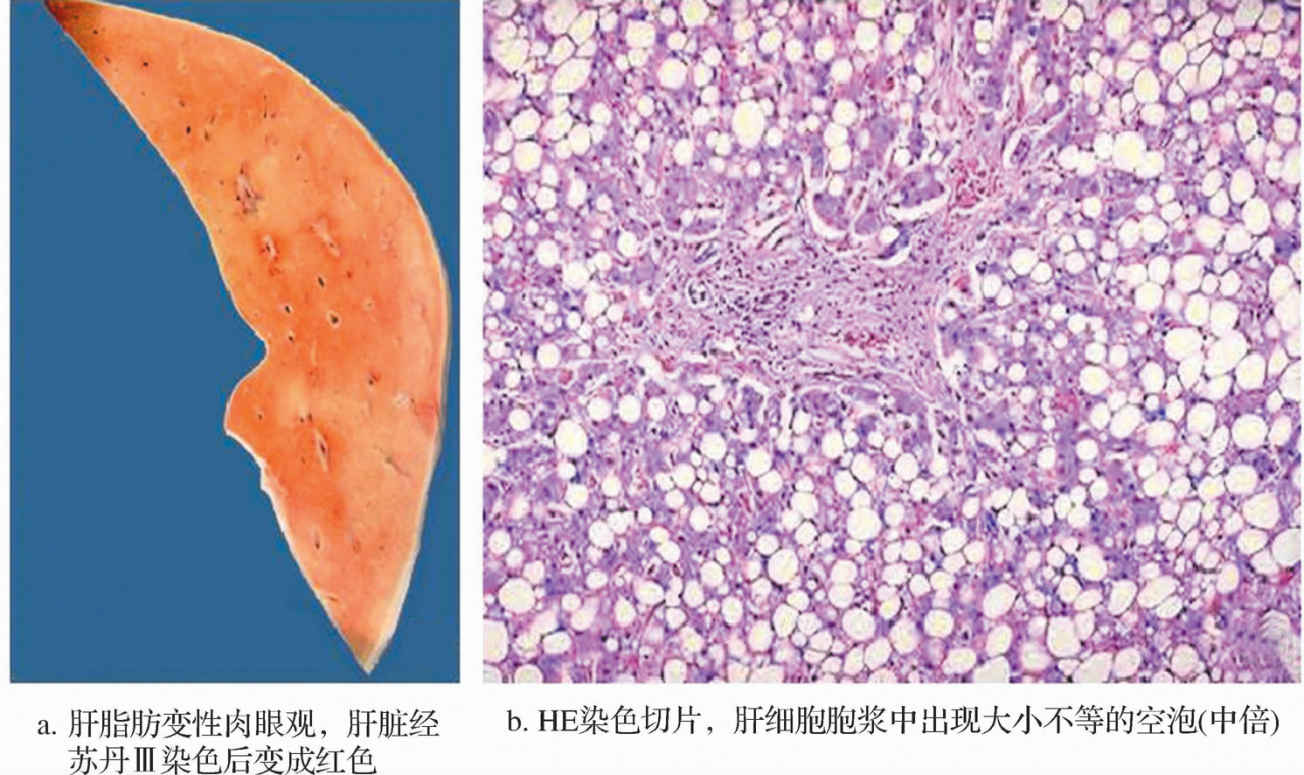
\includegraphics{./images/Image00009.jpg}
	\caption{肝脂肪变性}
	\label{fig1-8}
\end{figure}
%\FloatBarrier 



肝脂变是可复性损伤,病因消除后,脂变细胞可恢复正常,一般无明显的临床表现。重度弥漫性肝脂变称为脂肪肝,体检时肝可在右季肋下触及,常规B超可进行诊断。病变持续发展,肝细胞逐渐坏死,纤维组织增生,可发展为肝硬化。

(2)心肌脂肪变性:多见于贫血。肉眼观:轻度脂变一般无明显异常,但在严重贫血时,常在心内膜下,尤其是左心室乳头肌处出现红黄相间的条纹,如虎皮斑纹,称为“虎斑心”。这是由于心肌内血管分布不均,心肌缺氧轻重程度不一所致,血管末梢分布区心肌缺氧较重,脂变明显而呈黄色,缺氧较轻部位脂变较轻,心肌呈红色。镜下观:脂肪空泡常较细小,呈串珠状排列。有时心外膜增生的脂肪组织可沿间质深入心肌细胞间,称为心肌脂肪浸润(图\ref{1-9})。
\begin{figure}[!htbp]
	\centering
	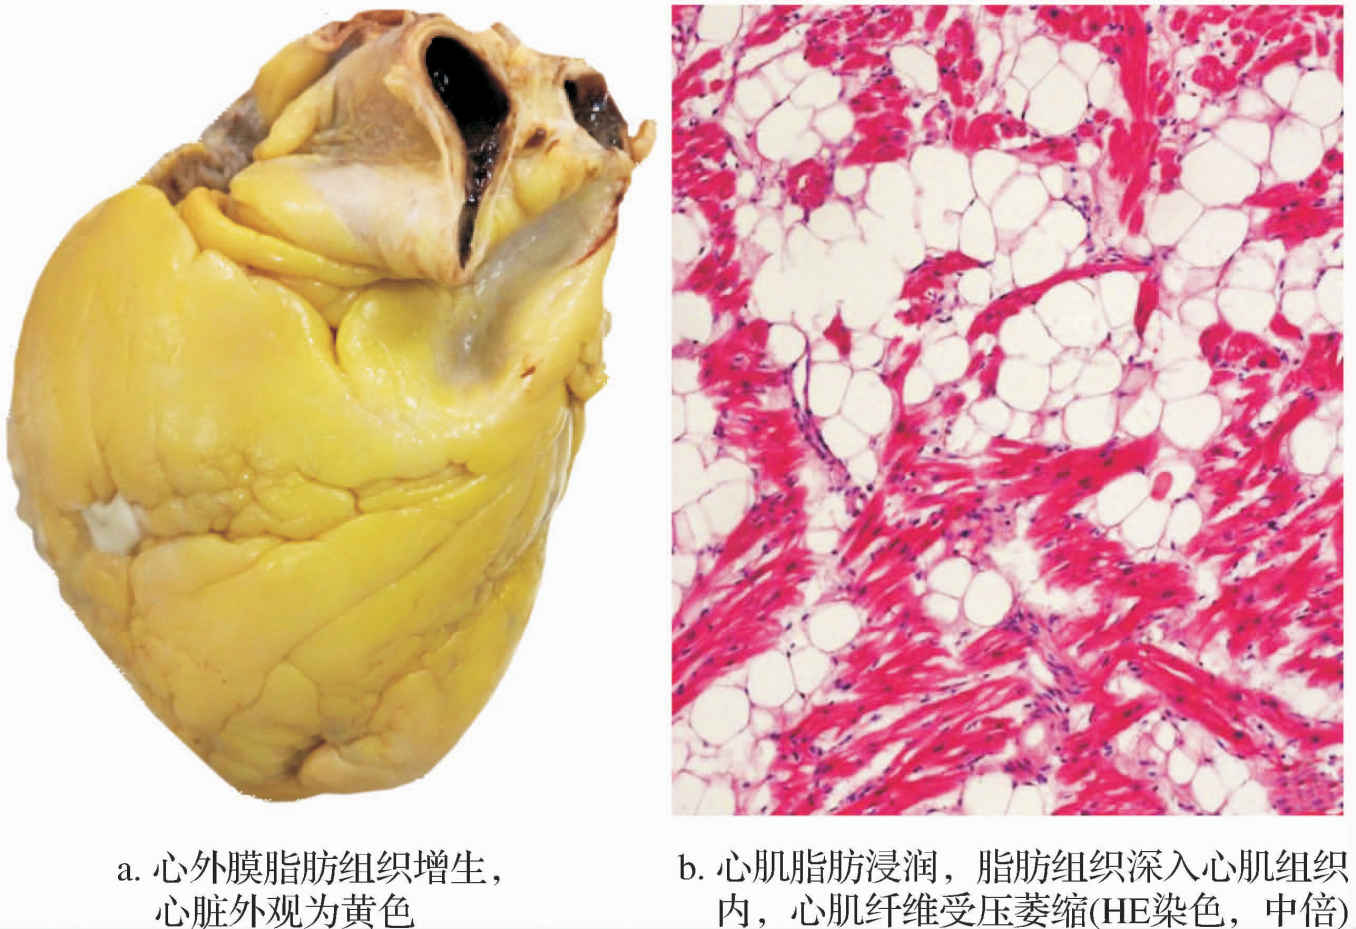
\includegraphics[width=0.7\textwidth]{./images/Image00010.jpg}
	\caption{心外膜脂肪组织增生及心肌脂肪浸润}
	\label{fig1-9}
\end{figure}
%\FloatBarrier 

(3)肾脂肪变性:贫血、缺氧、中毒和一些肾脏疾病时,肾曲管上皮细胞可发生脂肪变性。这是因为在上述疾病时肾小球毛细血管通透性增加,肾曲管特别是近曲小管上皮吸收漏出的脂蛋白,在细胞内分解成脂滴。脂滴空泡多位于近曲小管上皮细胞基底部或核周围。

脂肪变性发生的机制尚未完全清楚。一般认为与感染、中毒、缺氧等因素干扰或破坏细胞的脂肪代谢有关。具体作用途径则因病因不同而异。肝脂变的机制大致如下:①脂蛋白合成障碍,使脂肪堆积在肝细胞内不能转运出去。其原因常是缺乏合成脂蛋白的原料,如磷脂或组成磷脂的胆碱,或由于化学物或其他毒素破坏了内质网(蛋白合成部位)或抑制了某些酶的活性,使脂蛋白合成障碍。②脂肪酸氧化障碍。由于缺氧、感染、中毒,使线粒体受损,干扰β-氧化,使肝细胞含脂肪量增加。③进入肝细胞脂肪酸过多。例如饥饿或某些疾病造成饥饿状态,或糖尿病患者对糖的利用障碍,机体动用大量体脂,其中大部分以脂肪酸的形式进入肝脏,超过肝细胞将其氧化和合成脂蛋白的能力,于是在肝细胞内储积。

\paragraph{玻璃样变性}
玻璃样变性(hyaline
degeneration)又称透明变性,是指在HE染色情况下,细胞外间质或细胞质内出现伊红染、均质半透明、无结构的玻璃样物质。玻璃样变性其实为一组物理性状相同,但其发生原因、化学成分及机制各不相同的病理变化的统称。常见的玻璃样变性有三类:

(1)细胞内玻璃样变性:指细胞浆内出现大小不等、圆形、均质的红染小滴。细胞内玻璃样变性可由多种原因引起,如肾小球肾炎或其他疾病伴有明显蛋白尿时,肾近曲小管上皮细胞胞浆内可出现大小不等的圆形红染小滴,这是血浆蛋白经肾小球滤出而又被肾小管上皮细胞吞饮、融合而成的玻璃样小滴(图\ref{fig1-10}a)。慢性乙醇中毒时,由于细胞中间丝前角蛋白变性,肝细胞核周围的胞浆内可出现圆形或形状不甚规则的均质红染玻璃样物质,称为Mallory小体。

(2)结缔组织玻璃样变性:常发生在增生的纤维结缔组织,为胶原纤维老化的表现。肉眼观病变处呈灰白色,半透明,质地致密而坚韧(图\ref{fig1-10}b)。光镜下胶原蛋白交联、变性、融合,胶原纤维增粗并互相融合成索带状或片状的半透明均质物,纤维细胞明显减少。见于瘢痕组织、纤维化的肾小球、动脉粥样硬化的纤维斑块等。

(3)血管壁玻璃样变性:常发生于高血压病时的肾、脑、脾及视网膜的细动脉。这是由于细动脉持续痉挛,使内膜通透性增大,血浆蛋白渗入内膜,在内皮细胞下凝固成均匀红染玻璃样物质。如病变继续发展,血管壁平滑肌组织均被玻璃样物质替代而消失,再加上基底膜样物质增多,使病变血管壁增厚、变硬,管腔狭窄甚至闭塞,此即细动脉硬化症(图\ref{fig1-10}c),可引起肾、脑等器官缺血。
\begin{figure}[!htbp]
	\centering
	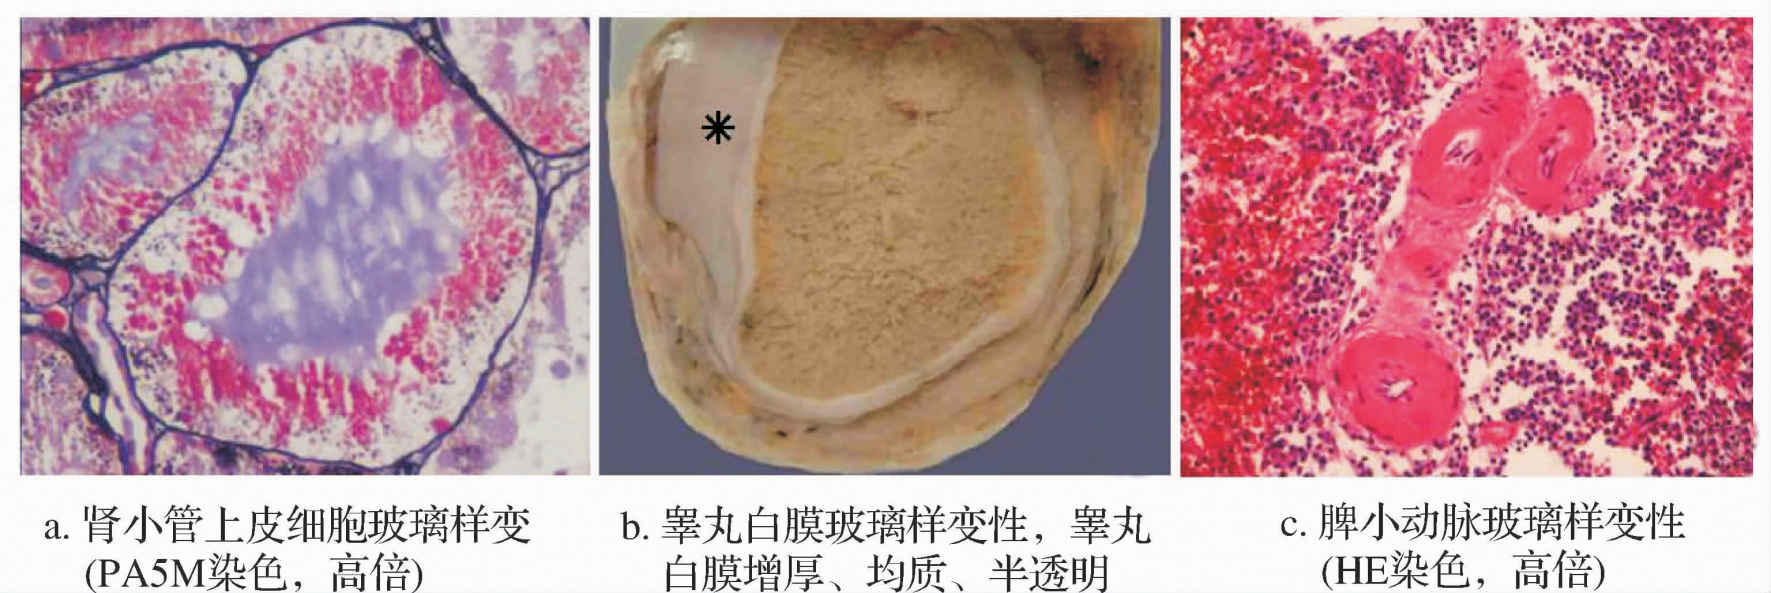
\includegraphics[width=0.7\textwidth]{./images/Image00011.jpg}
	\caption{不同类型玻璃样变性}
	\label{fig1-10}
\end{figure}
%\FloatBarrier

上述3种类型中,细胞内玻璃样变在病因去除后多能恢复,而后两者较难恢复。

\paragraph{黏液样变性}
组织间质内出现类黏液(黏多糖和蛋白质)的积聚称为黏液样变性(mucoid
degeneration)。镜下观:病变处细胞间质疏松,充以淡蓝色的胶状液体,其间散布一些多角形,星芒状的细胞,并以突起互相连缀。黏液样变性常见于间叶性肿瘤、急性风湿病时的心血管壁、动脉粥样硬化的血管壁。在甲状腺功能低下时,透明质酸酶活性受抑,含有透明质酸的黏液样物质及水分在皮下蓄积,形成黏液水肿。

\paragraph{淀粉样变}
组织内有淀粉样物质沉着称为淀粉样变(amyloid
degeneration)。淀粉样物质是蛋白质,其遇碘时可被染成棕褐色,再加硫酸后则变为蓝色,与淀粉染色特性相似,故称之为淀粉样变。此种病变可见于慢性炎症、内分泌系统肿瘤、老年性痴呆(Alzheimer病)等多种疾病。淀粉样物质的沉积可为局部性,亦可为全身性,常分布于细胞间或沉积在小血管基底膜下,还可沿组织纤维支架分布。镜下观:淀粉样物质呈淡伊红染色、均匀一致、云雾状。刚果红染色为橘红色(图\ref{fig1-11})。尽管形态相似,但在不同疾病时,淀粉样物质的化学本质不同,有的为免疫球蛋白,有的为激素,还有的为β{2}
淀粉样蛋白,等等。

\begin{figure}[!htbp]
	\centering
	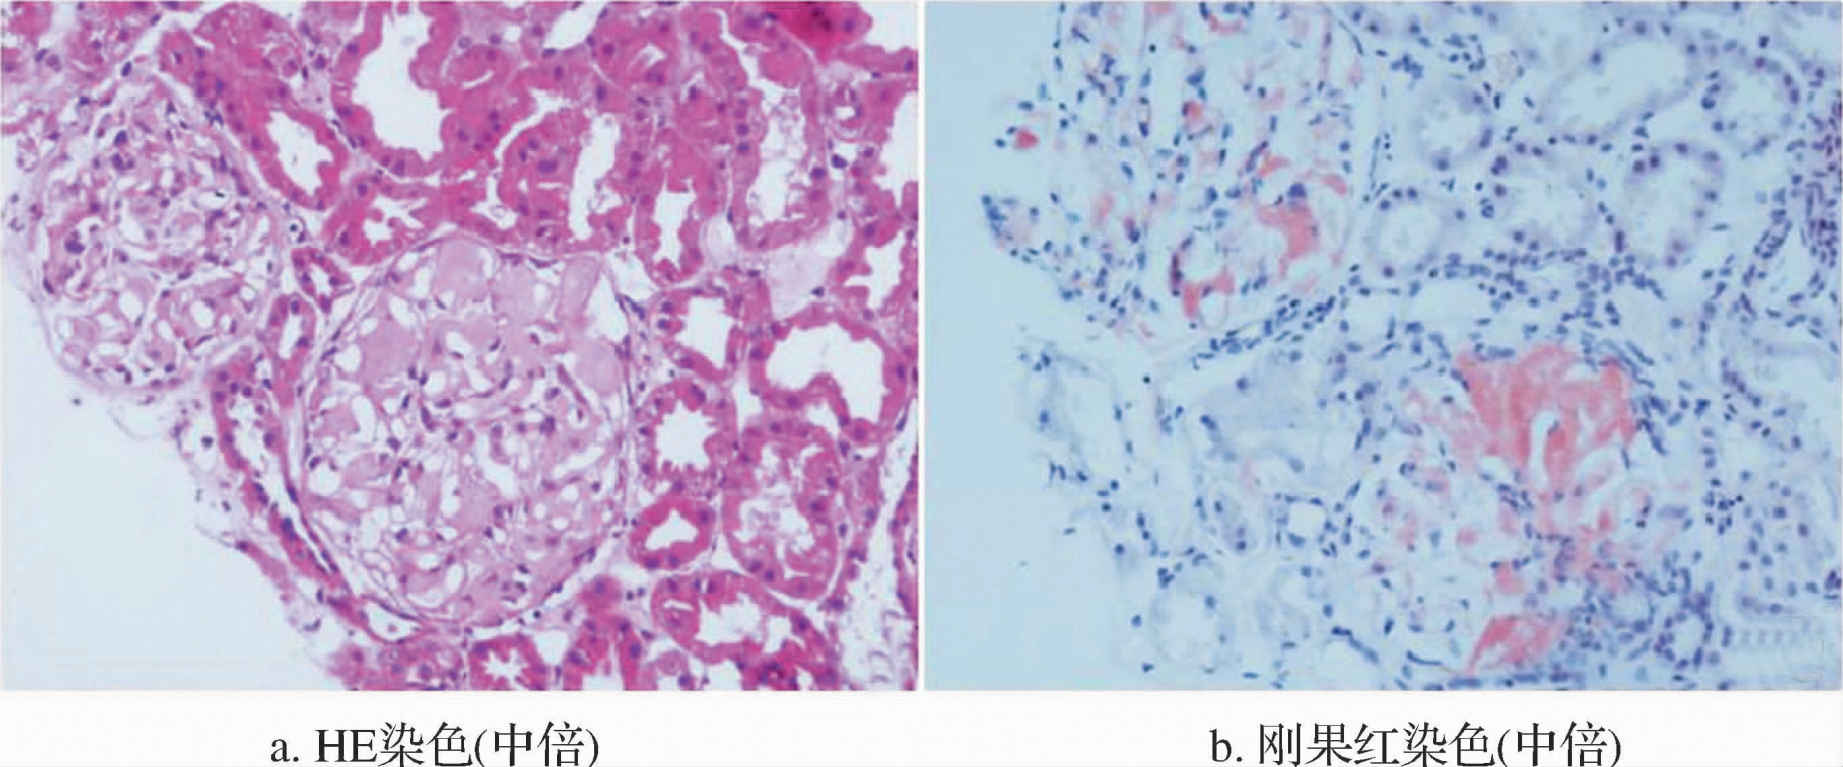
\includegraphics[width=0.7\textwidth]{./images/Image00012.jpg}
	\caption{肾小球淀粉样变}
	\label{fig1-11}
\end{figure}
%\FloatBarrier

\paragraph{病理性色素沉积}
细胞或组织内可有各种来自体内、体外的色素沉积,在病理情况下某些色素在体内会过量沉积。常见的病理性色素沉积有含铁血黄素、胆红素、脂褐素、黑色素。

(1)含铁血黄素(hemosiderin):系由铁蛋白微粒积聚而成的色素,颗粒状,棕黄或金黄色,具有折光性。此色素为血红蛋白被吞噬细胞溶酶体分解而成,如巨噬细胞破裂,则色素逸出于间质中。正常的骨髓组织或脾内可有少量含铁血黄素出现,在全身溶血性疾病时,含铁血黄素可沉积在全身的单核巨噬细胞系统内,组织出血时含铁血黄素常出现在出血灶附近。当左心衰竭导致肺淤血时,红细胞自肺泡壁毛细血管漏出于肺泡中,被巨噬细胞吞噬,肺泡腔内可出现吞噬含铁血黄素的巨噬细胞,又称为心力衰竭细胞。

(2)胆红素(bilirubin):也是在巨噬细胞内形成的一种血红蛋白衍生物,棕黄色或黄绿色。生理情况下,胆红素是衰老的红细胞被单核吞噬细胞分解后所形成。血中胆红素过多时,可将组织和体液染成黄色,称黄疸。因有血脑屏障,胆红素通常不能进入脑和脊髓,但在新生儿由于血脑屏障尚不完善,溶血性黄疸时,大量胆红素可进入脑细胞内,使其氧化磷酸化过程受损,能量产生受抑制,导致细胞变性,出现相应的神经症状。肉眼见豆状核、下丘脑、海马回等多处神经核明显黄染,故称之为核黄疸。胆红素一般呈溶解状态,但在胆道阻塞及某些肝脏疾病时也可为黄褐色折光性颗粒或团块,出现于肝细胞、Kupffer细胞、毛细胆管、小胆管等组织细胞内。

(3)脂褐素(lipofuscin):为一种黄褐色细颗粒状色素。其组成成分的50%为脂质,其余为蛋白质及其他物质。脂褐素系细胞内自噬溶酶体中的细胞器碎片发生了某种理化改变,不能被溶酶体酶消化而形成的一种不溶性残存小体。老年人及一些慢性消耗性疾病患者的肝细胞、肾上腺皮质网状带细胞和心肌细胞核两端的胞浆中可见到脂褐素,故又有消耗性色素之称。

(4)黑色素(melanin):为棕褐色或黑褐色的颗粒状色素,大小形状不一。正常人黑色素多存在于皮肤、毛发、虹膜及脉络膜的黑色素细胞内。它是由酪氨酸在黑色素细胞内的酪氨酸酶的作用下氧化、聚合而形成的一种不溶性聚合体。人脑垂体所分泌的ACTH能刺激黑色素细胞,促进黑色素形成。在肾上腺皮质功能低下时,对垂体的反馈抑制作用减弱,致使ACTH分泌增多,患者全身皮肤黑色素增多。局部黑色素增多常见于黑色素痣或恶性黑色素瘤等。

\paragraph{病理性钙化}
在病理情况下,骨和牙以外的组织内有固体钙盐的沉积,称为病理性钙化(pathologic
calcification)。主要成分为磷酸钙、碳酸钙及少量铁镁等物质。肉眼观:少量钙盐沉积难以辨认,仅在刀切组织时有砂粒感;量多时表现为白色石灰样颗粒或团块,质地坚硬。镜下观:HE染色切片中,钙盐呈蓝色颗粒状。病理性钙化可分为两种类型:

(1)营养不良性钙化:指钙盐沉积于变性、坏死的组织中或异物内,如结核坏死灶、脂肪坏死灶、动脉粥样硬化斑块的变性坏死区(图\ref{fig1-12}a),血栓、寄生虫体和虫卵。患者无全身钙、磷代谢障碍,血钙不高。这是一种较常见的病理性钙化,可能与局部碱性磷酸酶(来自坏死细胞及其周围组织内)升高有关。

\begin{figure}[!htbp]
	\centering
	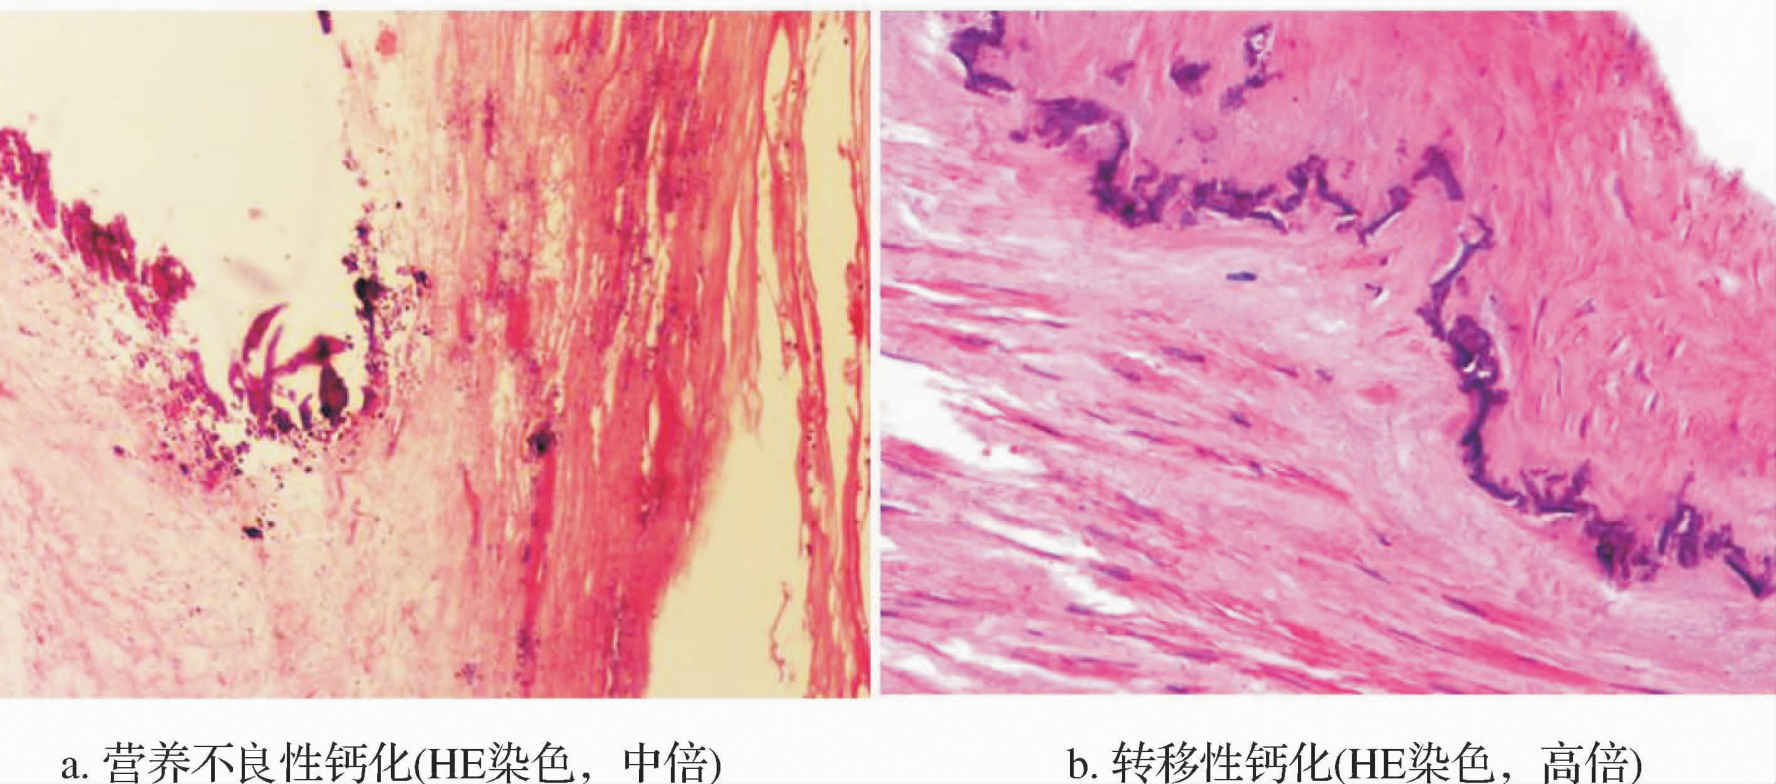
\includegraphics[width=0.7\textwidth]{./images/Image00013.jpg}
	\caption{动脉壁钙化}
	\label{fig1-12}
\end{figure}
%\FloatBarrier

(2)转移性钙化:较少见,是指由于全身钙、磷代谢障碍,血钙和(或)血磷升高,钙盐沉积于未受损的组织中。如甲状腺功能亢进或骨肿瘤造成骨组织破坏时,大量骨钙进入血液,使血钙升高,并沉积于肾小管、肺泡、胃黏膜和动脉壁中层(图\ref{fig1-12}b)。接受超剂量维生素D时,由于肠道对钙磷吸收明显增加,也可引起钙化。

钙化对机体的影响视具体情况而异。坏死组织钙化常是病灶愈合的表现,而血管壁的钙化则使管壁失去弹性、变硬、变脆,容易破裂出血。转移性钙化的危害性主要决定于原发病。

\subsubsection{不可逆性损伤-细胞死亡}

当细胞发生不可逆性代谢、结构和功能障碍,则引起细胞死亡(cell
death)。细胞死亡是病理学核心问题,其表现有两种方式:坏死与凋亡。坏死是细胞受到严重损伤时的病理性死亡过程,而凋亡多属生理性情况下发生的死亡,由细胞基因编程调控,在某些病理情况下,细胞死亡也可以凋亡形式出现。

\paragraph{坏死}
坏死(necrosis)是细胞受到严重损伤,以酶溶性变化为特点的活体内局部组织细胞的死亡。坏死可迅速发生,但在多数情况下由可逆性损伤逐渐发展而来。基本表现为细胞肿胀、细胞器崩解和蛋白质变性。

(1)坏死的基本病变

1)细胞核的改变:这是细胞坏死在形态学上的主要标志,表现为:①核浓缩(pyknosis),由于核脱水使染色质浓缩,嗜碱性染色增强,核体积缩小。②核碎裂(karyorrhexis),核染色质崩解为小碎片,核膜破裂,染色质碎片分散在胞质中。③核溶解(karyolysis),在DNA酶的作用下,染色质DNA分解,核乃失去对碱性染料的亲和力,因而染色变淡,仅见核轮廓,最后核消失(图\ref{fig1-13})。

\begin{figure}[!htbp]
	\centering
	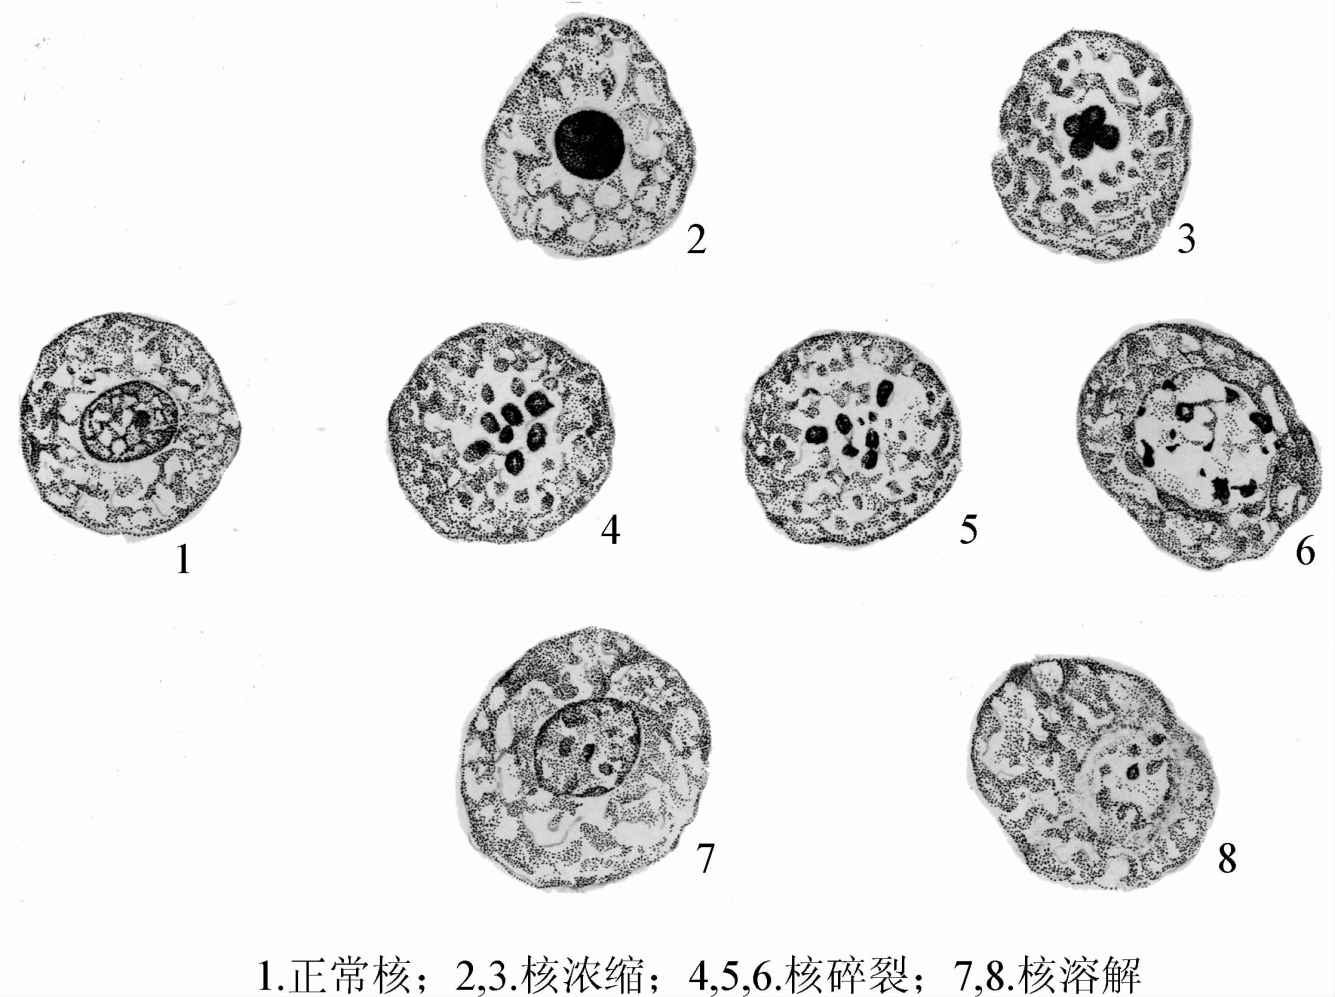
\includegraphics[width=0.7\textwidth]{./images/Image00014.jpg}
	\caption{细胞坏死时核的变化}
	\label{fig1-13}
\end{figure}

2)细胞浆的改变:由于细胞浆内嗜碱性核蛋白体减少或丧失,胞质变性蛋白质增多、糖原颗粒减少,使胞质对碱性染料苏木素的亲和力减少,而与酸性染料伊红的亲和力增强,致胞浆红染,坏死后期细胞浆崩解。

3)间质的改变:在实质细胞坏死后一段时间内,间质常无改变,以后在溶解酶的作用下,基质崩解,胶原纤维肿胀、断裂,继而崩解、液化。最后坏死的实质细胞和间质融合成一片无结构的颗粒状、红染物质,其内有时可见少量淡染的细胞核碎片。

由于坏死时细胞膜通透性增加,细胞内乳酸脱氢酶、琥珀酸脱氢酶、肌酸激酶、门冬氨酸氨基转移酶、丙氨酸氨基转移酶等被释放入血,造成细胞内酶活性降低而血浆中相应的酶活性升高,分别可作为诊断某些细胞(如肝、心肌、胰)坏死的参考指标。细胞内和血浆中酶活性的变化在坏死初即可检出,有助于细胞损伤早期诊断。

(2)坏死的病理类型:组织坏死后,由于酶的分解和蛋白质变性等因素综合作用的结果,使坏死组织出现不同的形态学变化,总体上可分为凝固性坏死、液化性坏死和特殊类型坏死等三个基本类型。

1)凝固性坏死(coagulation
necrosis):组织坏死后,蛋白质变性凝固且溶酶体酶水解作用较弱时,坏死区呈灰黄、干燥、质实状态,称为凝固性坏死。这种坏死多由缺血引起,常在心、肾、脾等器官的缺血性坏死时出现。
坏死灶周围常有暗红色出血带,与健康组织分界(图\ref{fig1-14}a)。
镜下特点:早期坏死灶细胞微细结构消失,但细胞组织的结构轮廓仍可保留一段时间(图\ref{fig1-14}b)。
最终坏死细胞崩解成碎片,被吞噬细胞吞噬或被游走进入的白细胞释放的溶解酶溶解。
凝固性坏死的发生机制仍不很清楚,可能是组织坏死后蛋白变性过程占优势,而水解酶的作用较少。

\begin{figure}[!htbp]
	\centering
	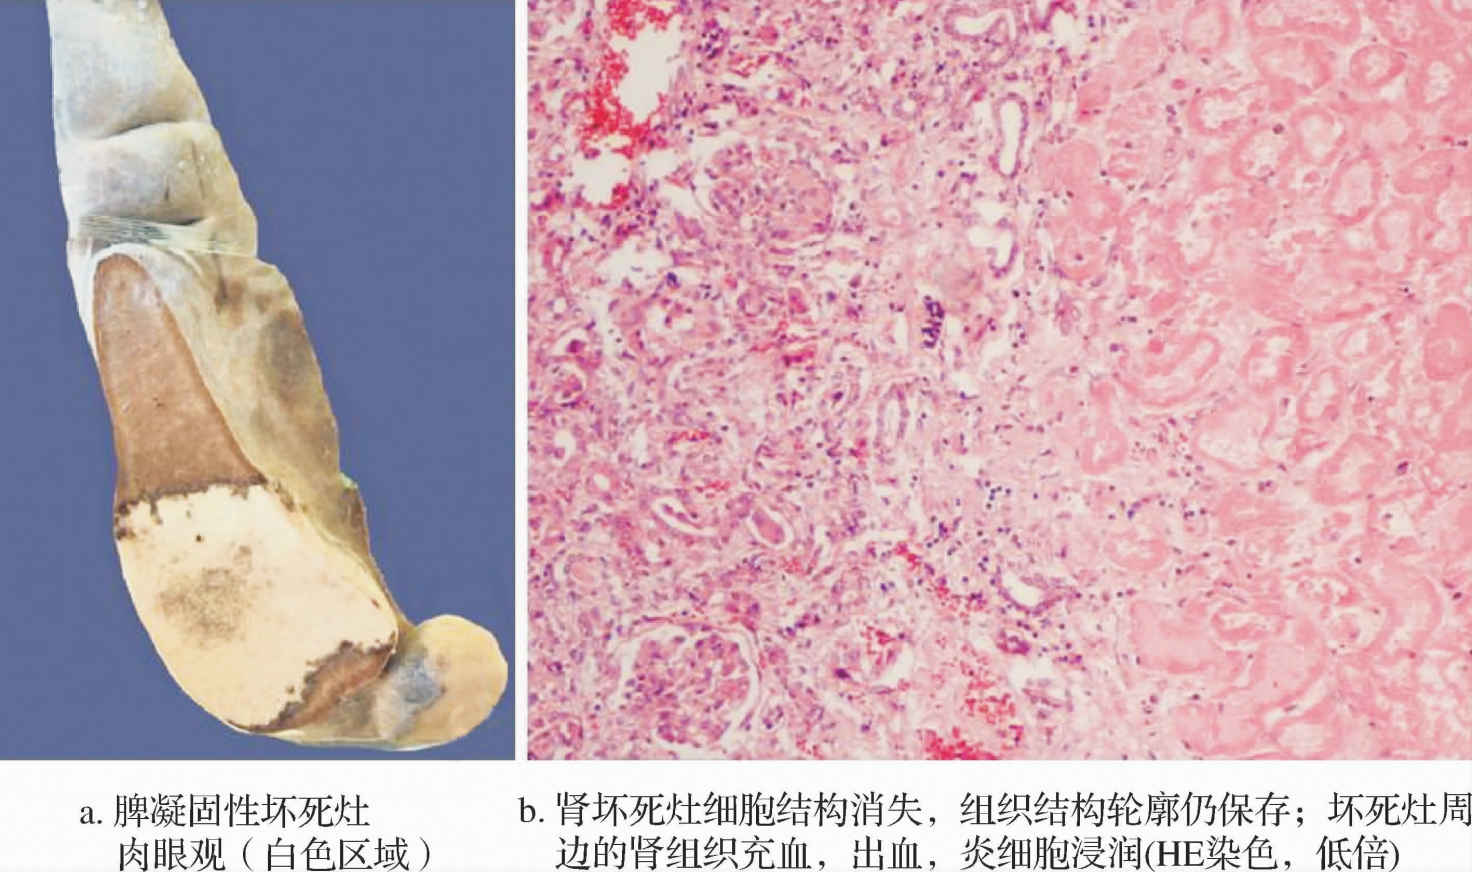
\includegraphics[width=.7\textwidth]{./images/Image00015.jpg}
	\caption{凝固性坏死}
	\label{fig1-14}
\end{figure}

2)液化性坏死(liquefaction
necrosis):组织坏死后分解、液化而呈液体状,有时还形成含有液体的腔。
如脑组织,坏死后分解成半流体状物质,又称为脑软化。
这种变化与脑组织水分和磷脂含量多,蛋白质含量少有关,故组织坏死后不易凝固而液化。
在某些病原体如化脓性细菌或溶组织阿米巴原虫能释放或产生蛋白溶解酶,可使组织发生液化性坏死。

3)特殊类型坏死

①干酪样坏死(caseous
necrosis):结核病时,坏死区内脂质较多,颜色带黄,质地松软,状似干酪,故称为干酪样坏死。
镜下观:坏死组织分解比较彻底,原有组织轮廓消失,呈现为一片红染、无定形的颗粒状物质(图\ref{fig1-15})。
梅毒性的坏死组织具有相似的形态,但其中的弹力纤维及血管结构仍可保留,致使坏死组织质地坚韧如树胶,故名树胶肿。
干酪样坏死不易吸收,一旦形成将存留较长时间。

\begin{figure}[!htbp]
	\centering
	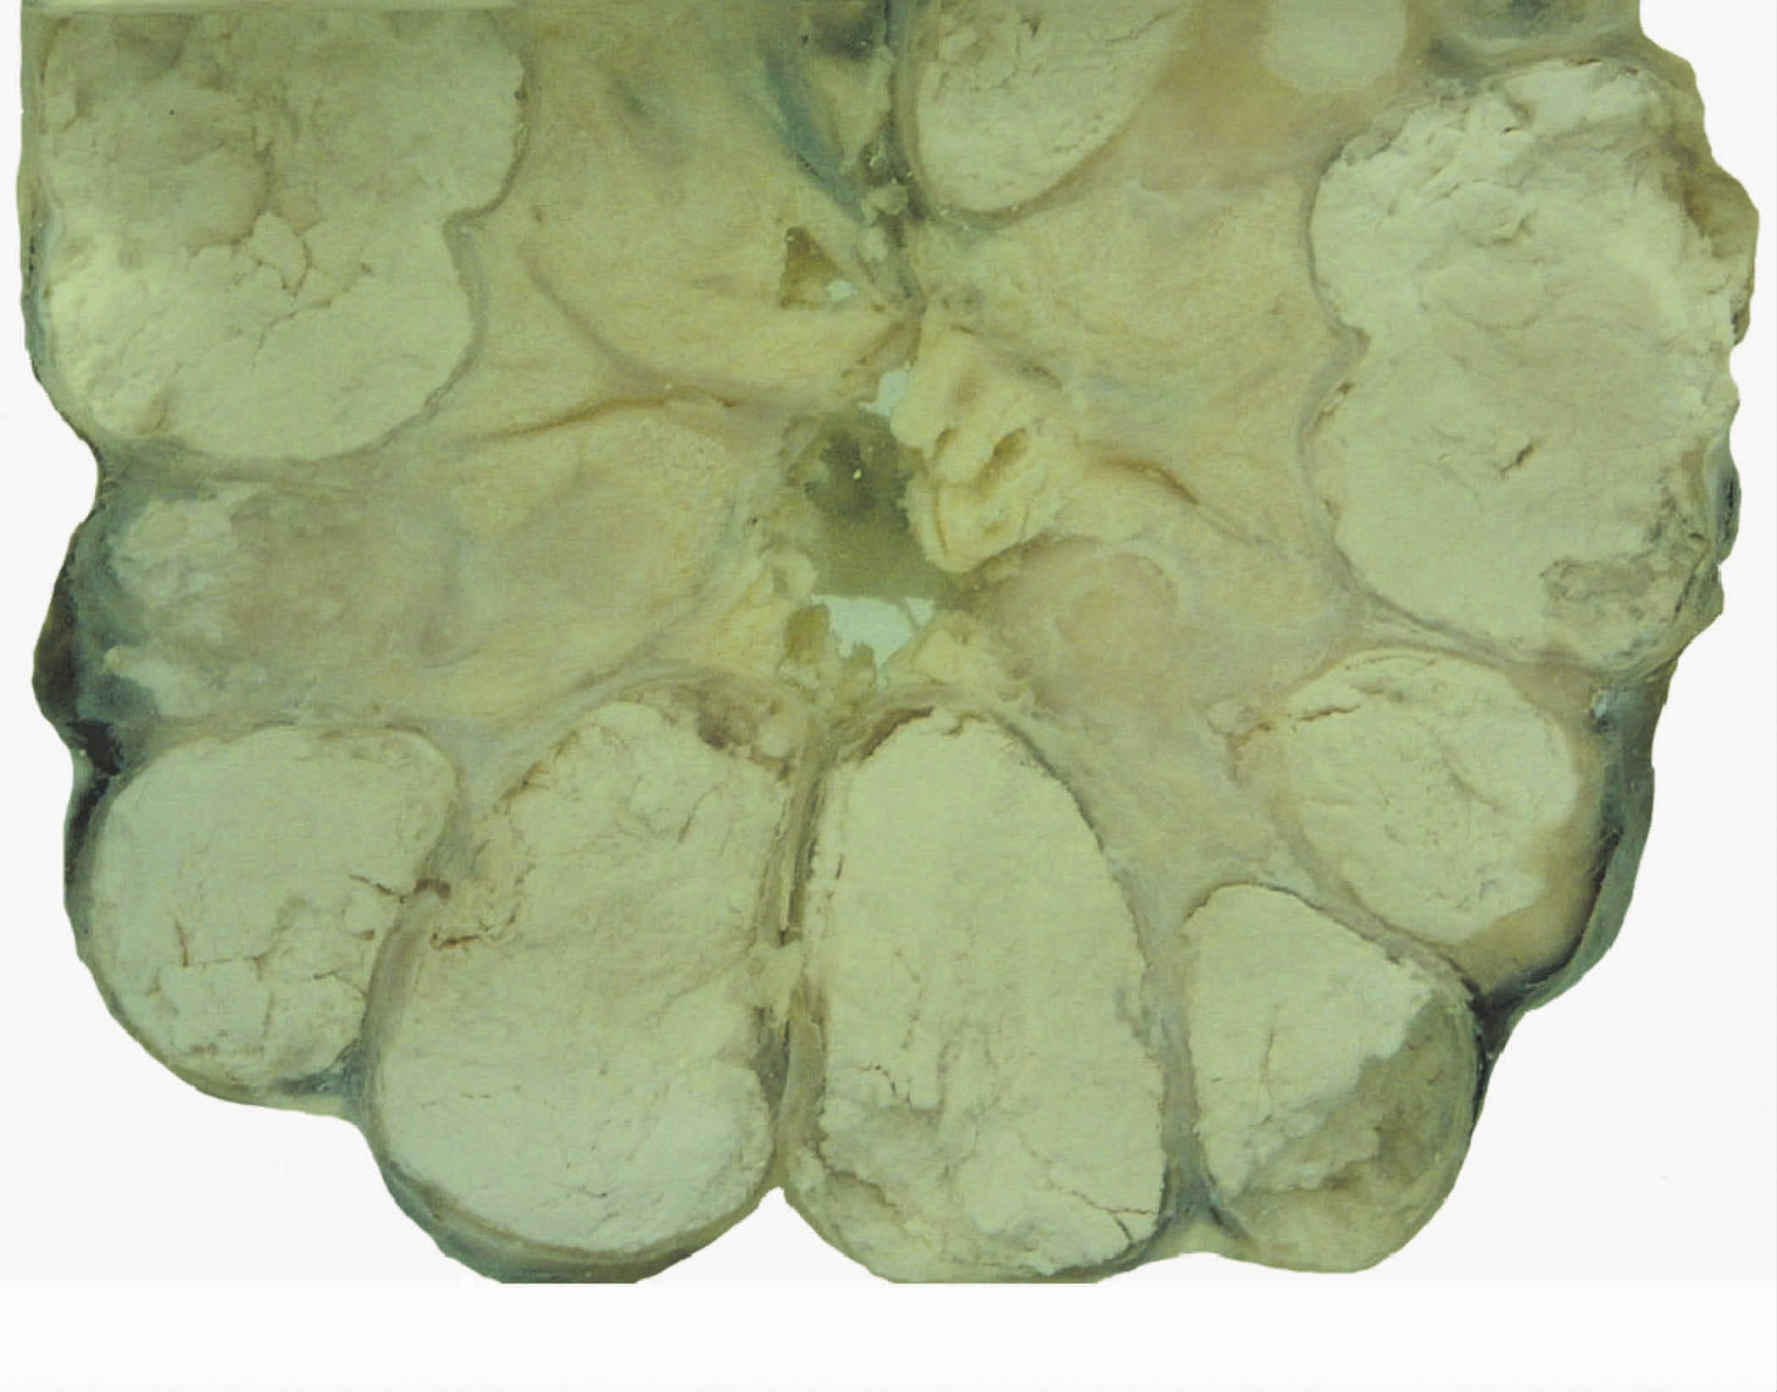
\includegraphics{./images/Image00016.jpg}
	\caption{肾干酪样坏死 \\ {\small 肾剖面可见多个黄白色干酪样坏死灶。}}
	\label{fig1-15}
\end{figure}

②纤维素样坏死(fibrinoid necrosis):旧称纤维素样变性(fibrinoid
degeneration)为发生于结缔组织胶原纤维和小血管壁的一种坏死。病变部位组织结构逐渐消失,变为一片境界不清的颗粒状、小条状或小块状无结构物质,经伊红染成深红色,由于其与纤维素染色性质相似,故名。常见于风湿病、结节性多动脉炎、新月体性肾小球肾炎、系统性红斑性狼疮等变态反应性疾病(图\ref{fig1-16})。也可见于恶性高血压病时的细动脉和胃溃疡底部动脉壁。其发生机制与抗原-抗体复合物引发的胶原纤维肿胀崩解、结缔组织免疫球蛋白沉积或血液纤维蛋白渗出变性有关。

\begin{figure}[!htbp]
	\centering
	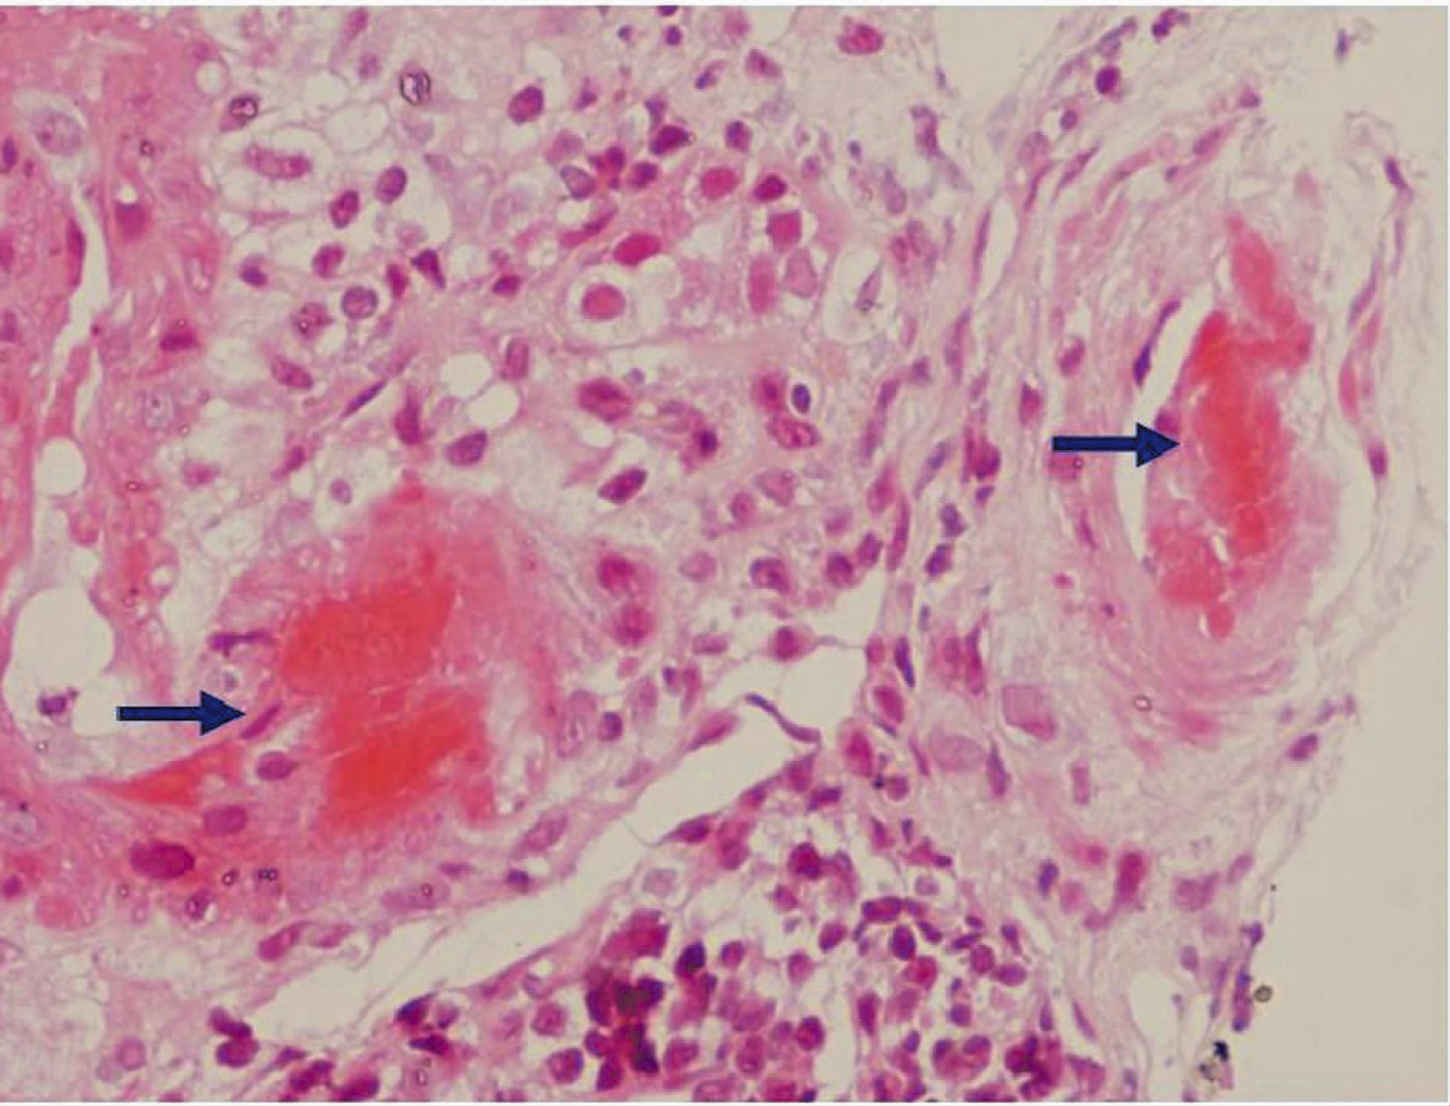
\includegraphics{./images/Image00017.jpg}
	\caption{肾小动脉壁纤维素样坏死(HE染色,高倍) \\ {\small 箭头所示深伊红染区为小动脉壁纤维素样坏死。}}
	\label{fig1-16}
\end{figure}


③脂肪坏死(fatty
necrosis):为液化性坏死的一种特殊类型,又可分为酶解性脂肪坏死和外伤性脂肪坏死。
前者常见于急性胰腺炎,由于胰脂酶外逸并被激活,对胰腺自身及腹腔的脂肪组织发生分解作用,形成的脂肪酸与组织内钙盐结合,在大网膜、后腹壁及肠系膜表面形成灰白色、质硬的不透明斑点或斑块,称为皂钙。
外伤性脂肪坏死常发生于富于脂肪组织的部位,乳腺尤其多见,有外伤史,局部表现为增大的肿块。镜下为大量的泡沫细胞及异物巨细胞。

④坏疽(gangrene):大块组织坏死后继发腐败菌感染,出现不同程度的腐败性变化。
腐败菌在分解坏死组织的过程中产生大量的硫化氢,并与血红蛋白分解释出的铁离子结合,形成硫化亚铁,致使坏死组织臭而发黑。
根据坏疽发生的部位、原因及形态特征不同,可分为干性、湿性、气性等类型。
干性坏疽(dry
gangrene)多发生于动脉阻塞而静脉回流仍然通畅的四肢末梢,坏死局部干燥、皱缩,呈黑色,与周围组织分界清楚(图\ref{fig1-17}),腐败性变化较轻。
湿性坏疽(moist
gangrene)常发生于与体外相连的内脏,如肠、阑尾等器官,也可发生于四肢。
形成的原因除动脉阻塞外,同时伴有局部淤血,坏死组织含水量多,适合腐败菌生长。
坏死区局部明显肿胀,呈深黄、暗绿或污黑,与周围组织无明显分界线,可引起严重的全身中毒症状。气性坏疽(gas
gangrene)也属于湿性坏疽。系深达肌肉的开放性创伤合并产气荚膜杆菌、腐败弧菌等厌氧菌感染。
细菌在分解液化组织的过程中产生大量气体,使坏死组织呈蜂窝状,压之有捻发感。
病变发展迅猛,沿肌束迅速蔓延。由于大量毒素被吸收,患者中毒症状十分严重,常需要紧急处理。

\begin{figure}[!htbp]
	\centering
	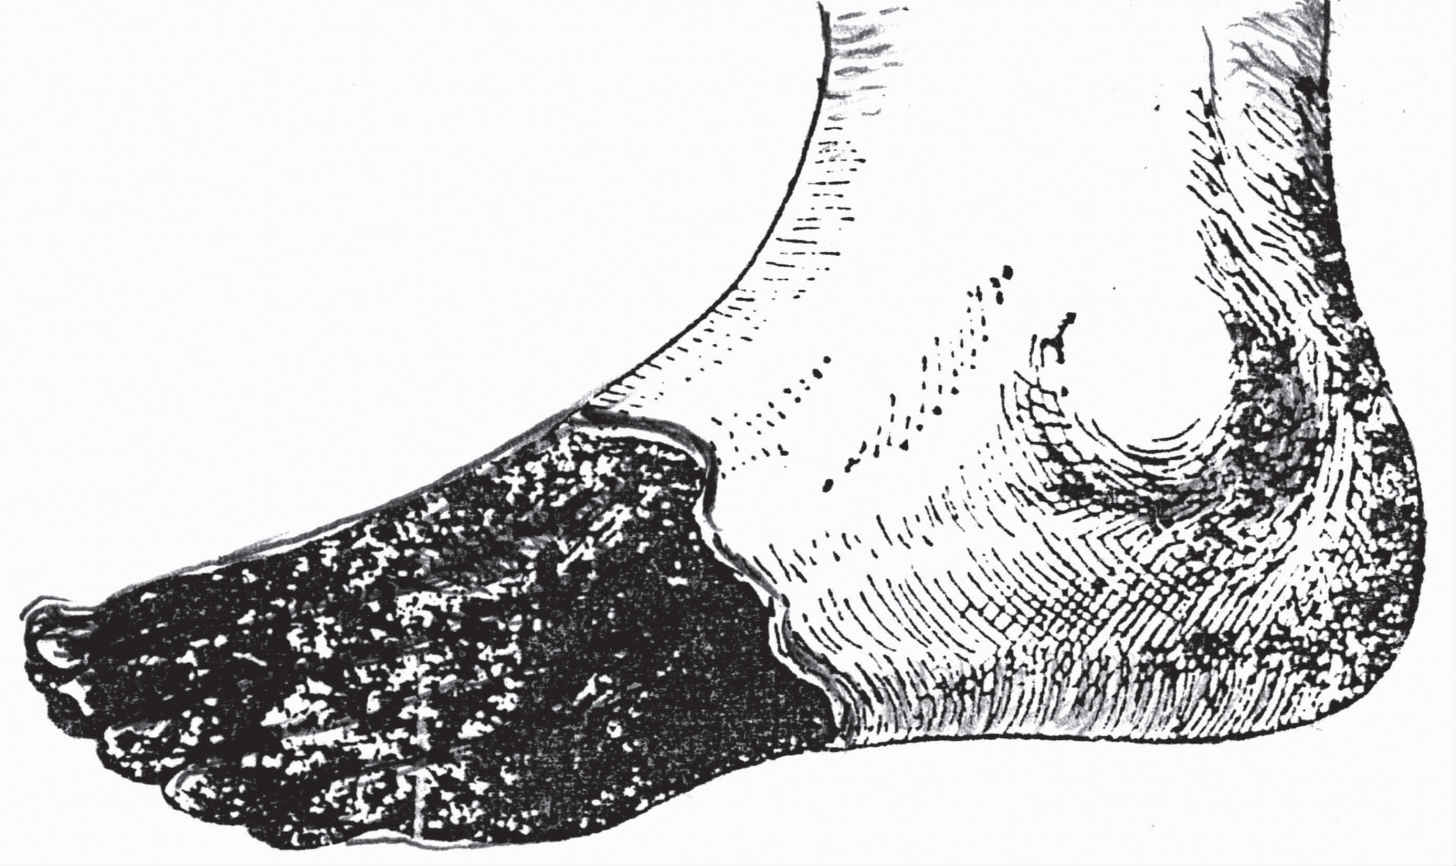
\includegraphics{./images/Image00018.jpg}
	\caption{足(干性)坏疽}
	\label{fig1-17}
\end{figure}

(3)坏死的结局:组织坏死后成了机体的异物,刺激周围组织,引起局部反应。不同的坏死组织结局不尽相同。

1)溶解吸收:坏死细胞自身或周围的炎细胞释放的溶解酶将坏死组织分解、液化,然后由淋巴管或小血管吸收,未被完全分解的组织碎片由吞噬细胞吞噬清除。坏死范围较大可形成囊腔。留下的组织缺损通过再生修复,这是机体处理坏死组织的基本方式。

2)分离排出:较大的坏死灶不易完全吸收,由于其周围发生炎症反应,其中的白细胞释放的溶解酶加速周边坏死组织溶解、吸收,使坏死灶与健康组织分离。位于皮肤、黏膜的坏死组织分离后脱落,留下局部缺损,浅者称为糜烂,深者称为溃疡。肾和肺脏的坏死组织分离后经自然管道排出,留下的空腔称为空洞。

3)机化与纤维包裹:坏死组织如不能被溶解吸收或分离排出,则由周围新生的毛细血管和成纤维细胞(合称肉芽组织)逐渐长入,取代坏死组织,最后形成瘢痕组织。这种由肉芽组织取代坏死组织(或其他异物、血凝块、血栓及渗出物等)的过程称为机化(organization)。如果坏死灶较大,难以吸收、机化,周边部增生的肉芽组织可将坏死灶包围,尔后肉芽组织转变为纤维组织,称为纤维包裹。机化和包裹的肉芽组织最终形成纤维瘢痕。

4)钙化:坏死组织和细胞碎片若未被及时清除,则日后易发生钙盐及其他矿物质沉积,引起营养不良性钙化。陈旧性干酪样坏死病灶或坏死的脂肪组织常有明显的钙化。

\paragraph{细胞凋亡}
细胞凋亡(apoptosis)也称程序性细胞死亡,是真核细胞在一定条件下通过启动其自身内部机制,主要是激活内源性核酸内切酶而发生的细胞主动性死亡方式。与细胞坏死不同,凋亡是一种主动过程,通常为单个细胞或小灶性细胞死亡,而不是大片实质细胞同时死亡。凋亡细胞周围无炎症反应,故有人借用希腊词“apoptosis”来形容其像秋天枯萎的树叶,从树干上悄无声息地飘零下来。

(1)形态特征:凋亡细胞有独特的形态特征。早期表现为细胞变圆,微绒毛及细胞突起消失,同时胞质浓缩,内质网扩张呈泡状,并与细胞膜融合形成细胞质小泡,向外隆起但无膜破裂;核染色质浓缩、凝聚于核膜下呈半月形。而后细胞膜内陷,自行分割为数个由胞膜包裹的、表面光滑的凋亡小体,其中含有大小不等的染色质片断、结构尚保持完整的细胞器和胞质成分(图\ref{fig1-18})。凋亡小体可与周围细胞分离,很快被邻近的细胞或巨噬细胞吞噬,在胞质溶酶体内迅速降解。

\begin{figure}[!htbp]
	\centering
	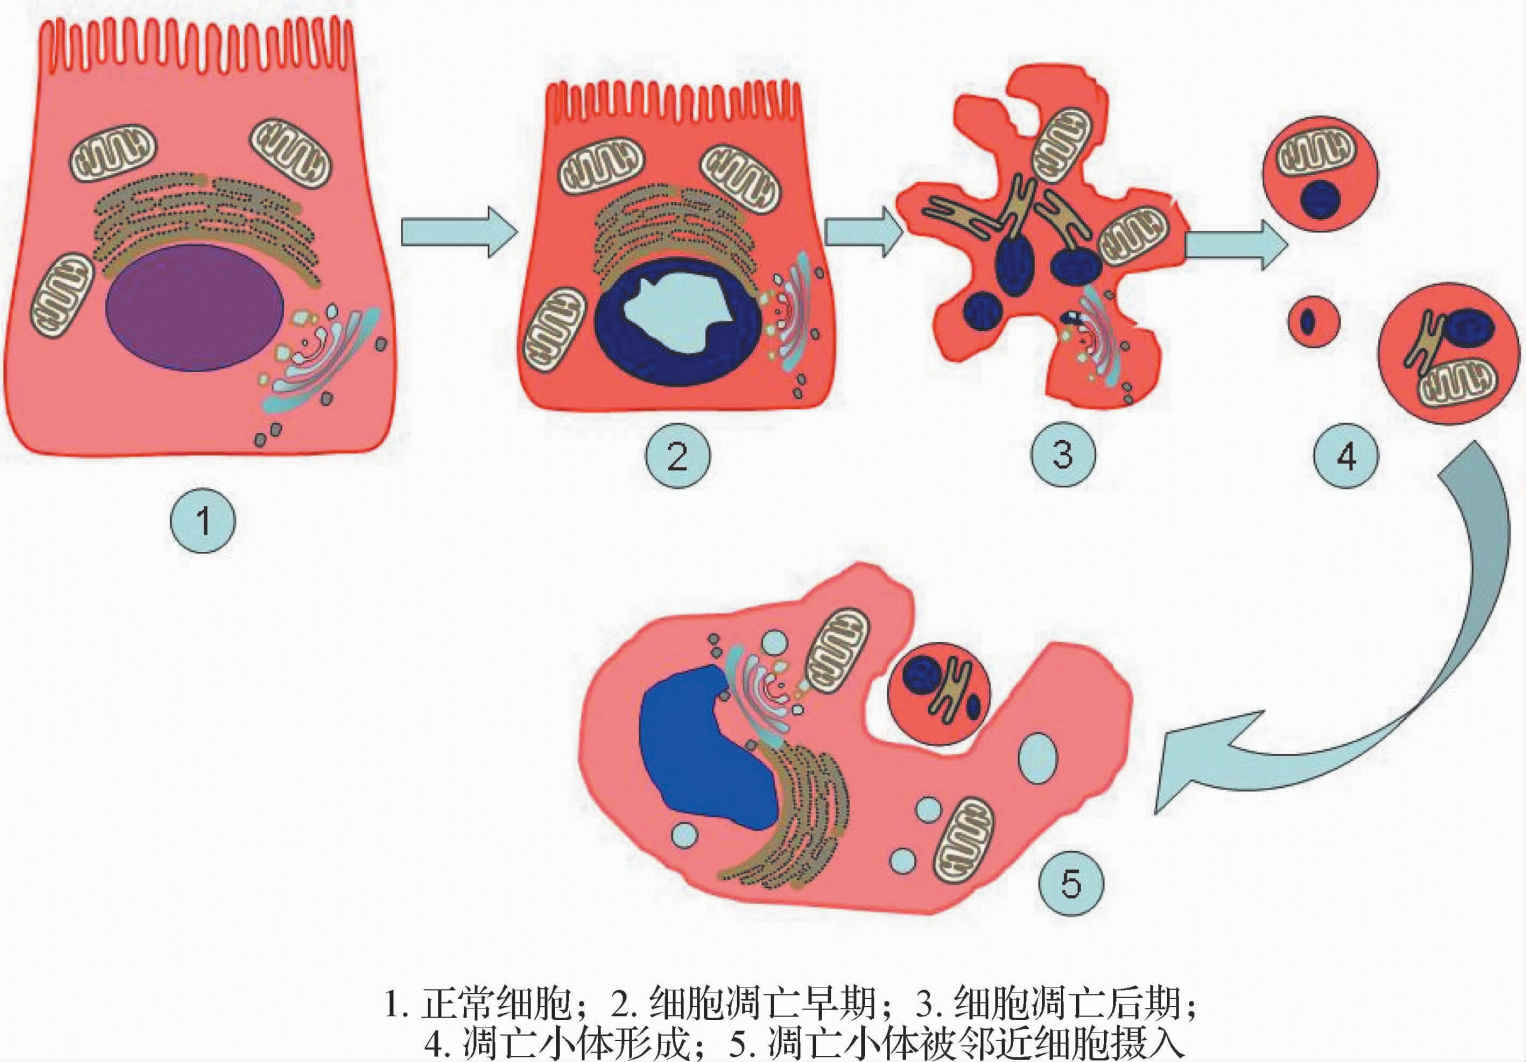
\includegraphics[width=.7\textwidth]{./images/Image00019.jpg}
	\caption{凋亡示意图}
	\label{fig1-18}
\end{figure}

(2)发生机制:细胞凋亡的发生机制十分复杂,它是一种由某些刺激因子启动、内在基因调控,并依赖能源的连锁分子事件,其中有信号传导、特异性调节分子作用、共同蛋白酶(caspases,半胱氨酸天冬氨酸蛋白酶,亦称胱冬肽酶)家族活化及死亡细胞的被噬和移去等过程,故曾有程序性死亡(programmed
cell death)之称。

刺激因子不同,其信号通路、调节分子种类不尽相同。目前已知,在人体各种病理过程中,发生细胞凋亡的主要通路有两条(图\ref{fig1-19}):一是线粒体通路或内源通路;二是死亡受体通路或外源通路。

\begin{figure}[!htbp]
	\centering
	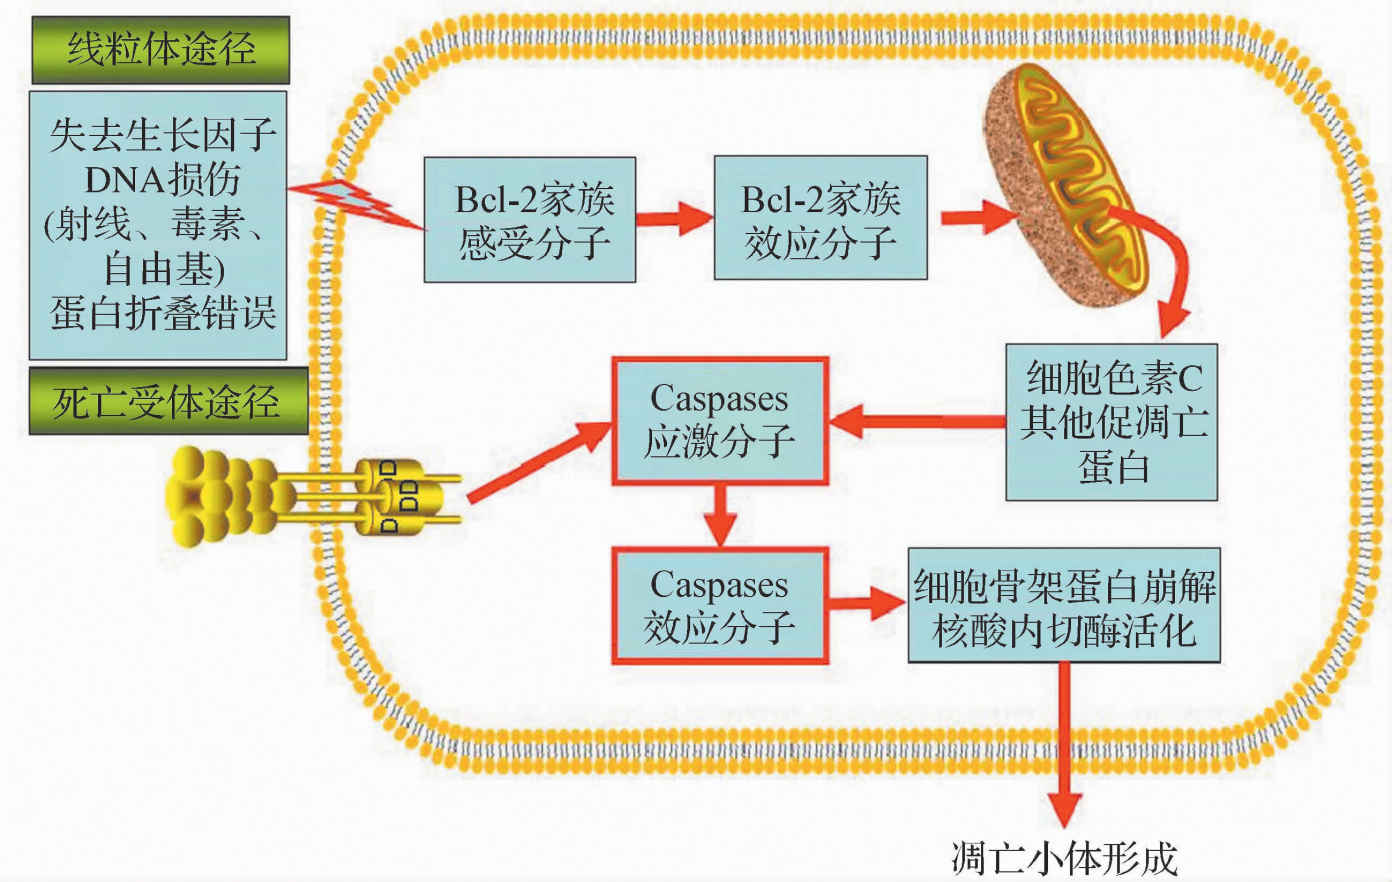
\includegraphics[width=.7\textwidth]{./images/Image00020.jpg}
	\caption{细胞凋亡机制示意图}
	\label{fig1-19}
\end{figure}

线粒体通透性决定细胞是否凋亡,而通透性受控于含20个以上蛋白成员的Bcl-2家族。当细胞失去生长因子或生存信号、暴露于DNA损伤因子(如紫外线、放射线、活性氧和细胞毒药物等)以及细胞内堆积过多的错误折叠蛋白时,Bcl-2家族感应分子即被活化,继之活化该家族另外两个成员(效应分子)-Bax和Bak,它们形成二聚体并插入线粒体膜,使后者通透性增加,细胞色素C和其他蛋白分子逸出线粒体进入胞浆,令激发性胱冬肽酶(caspase
9)活化,后者再使效应性胱冬肽酶(caspase
3、6、7)活化,最终导致细胞骨架蛋白崩解、核酸内切酶活化和凋亡小体形成。Bcl-2、Bcl-x{L}
抑制Bax和Bak活化,故可阻断凋亡。

细胞凋亡的死亡受体通路涉及肿瘤坏死因子(TNF)及其受体(TNFR)、FAS-FAS配体作用等。受体的胞内段为死亡功能区(dead
domain)。一旦受体配体结合,死亡信号即通过死亡功能区和相关的适配蛋白(adapter
protein)传递至激发性胱冬肽酶(caspase
8),并使之活化。后续反应与线粒体通路相同。

(3)细胞凋亡与坏死的区别:细胞凋亡的发生机制与前述的坏死不同,有相关基因调节。其中Fas、Bax、P53等基因有促进作用,Bcl-2、Bcl-x{L}
等有抑制凋亡作用。凋亡细胞内源性Ca{2+} 、Mg{2+}
依赖DNA内切酶的激活,从而切割核小体间DNA,形成不连续的180~200
bp或其倍数的DNA片断。被切割的DNA片断在琼脂糖凝胶电泳时表现为阶梯状电泳条带,这种现象被认为是细胞凋亡的可靠指标。凋亡的细胞质膜完整,无细胞内容物溢出,不引起细胞周围炎症反应,也不诱发周围细胞的增生修复。细胞凋亡和细胞坏死的区别见表\ref{tab1-1}。

\begin{table}[ht]
	\caption{细胞凋亡和细胞坏死的区别}
	\label{tab1-1}
	\centering
	\begin{tabular}{lp{5cm}p{5cm}}
		\toprule
		         & 细胞凋亡                                                                           & 细胞坏死                       \\
		\midrule
		形态特征 & 细胞固缩,核染色质边集、细胞膜及各细胞器膜完整,膜可发泡出芽,形成调亡小体
		         & 细胞显著肿胀,核染色质絮状或边集,细胞膜及各细胞器膜溶解破裂,溶酶体释放,细胞溶解                                  \\
		生化特征 & 核酸内切酶活化,半胱氨酸蛋白酶活化,谷氨酰谷氨酰转移酶活性增高
		         & 核酸内切酶无活化,半胱氨酸蛋白酶、转移酶活性无变化                                                                  \\
		DNA电泳  & 阶梯状条带                                                                         & 弥散分布的电泳拖带             \\
		炎症反应 & 无                                                                                 & 有                             \\
		机制     & 由凋亡相关基因调控主动进行(自杀性)                                                 & 与基因调控无关被动进行(他杀性) \\
		发生条件 & 多为生理性                                                                         & 病理性                         \\
		\bottomrule
	\end{tabular}
\end{table}


(4)细胞凋亡的生理、病理意义:细胞凋亡是最基本的生物现象,是机体生存和发育的基础。大量研究材料显示它涉及生命活动中的许多领域,包括发育、生长、造血、免疫、肿瘤发生等。通过凋亡可以清除多余的、无用的细胞。胚胎发育过程中,一些遗迹如人胚的尾芽和鳃随发育定期消亡,就是通过凋亡的方式进行的。细胞凋亡也可作为机体的自身保护机制,以清除发育不正常及对机体有害的细胞,畸胎瘤就是未彻底凋亡的残留胚层结构存留所致。B和T细胞发育成熟过程中本该发生凋亡的细胞保留下来将形成自身抗原,导致自身免疫病;细胞凋亡的异常改变包括凋亡不足或凋亡过度都可引起一些疾病。T辅助细胞($\text{CD}^+_4$
)在人类免疫缺陷病毒(HIV)感染后,发生凋亡,从而导致获得性免疫缺陷病。细胞凋亡的调控失常与肿瘤的发生关系密切,当机体某个基因发生突变而导致凋亡信号下调凋亡不足时,可引起细胞异常增生而发生肿瘤。目前临床上已开始用药物或放射线来诱导肿瘤细胞凋亡以达到治疗肿瘤的目的。

\begin{center}
	\textbf{知识链接}
\end{center}
\chapterabstract{自噬(autophagy)是细胞对自身细胞器或胞内聚集的变性蛋白等大分子物质进行包裹以及降解消化的现象。近年发现自噬不足或过度均可导致细胞死亡,所以被称为第三种细胞死亡方式。}

生理状态下,细胞通过自噬来清除受损、衰老和失去功能的细胞器及各种大分子物质,最终降解产物再循环利用,为细胞重建和再生提供原料。病理状态下,自噬不仅能保护细胞免受毒物损伤,而且能抵御病原体的侵害。在机体的免疫、感染、炎症、肿瘤、心血管病和神经退行性疾病的发生发展过程中均发挥重要作用。自噬和凋亡有相似之处,如二者共享某些调节蛋白,如胱冬肽酶。某些刺激因素既可诱导自噬亦可引起凋亡。

总之,疾病源于组织细胞的损伤,内外因子的刺激强度不同,损伤程度不同(图\ref{fig1-20})。若刺激在细胞能承受范围内,则表现为适应,属轻度损伤,细胞可出现萎缩、增生、肥大和化生等形态学改变。若刺激时间长强度大,细胞将发生显著损伤,出现细胞内外异常物质沉积,甚至坏死;若刺激因素激活特殊信号系统,细胞可发生凋亡。

\begin{figure}[!htbp]
	\centering
	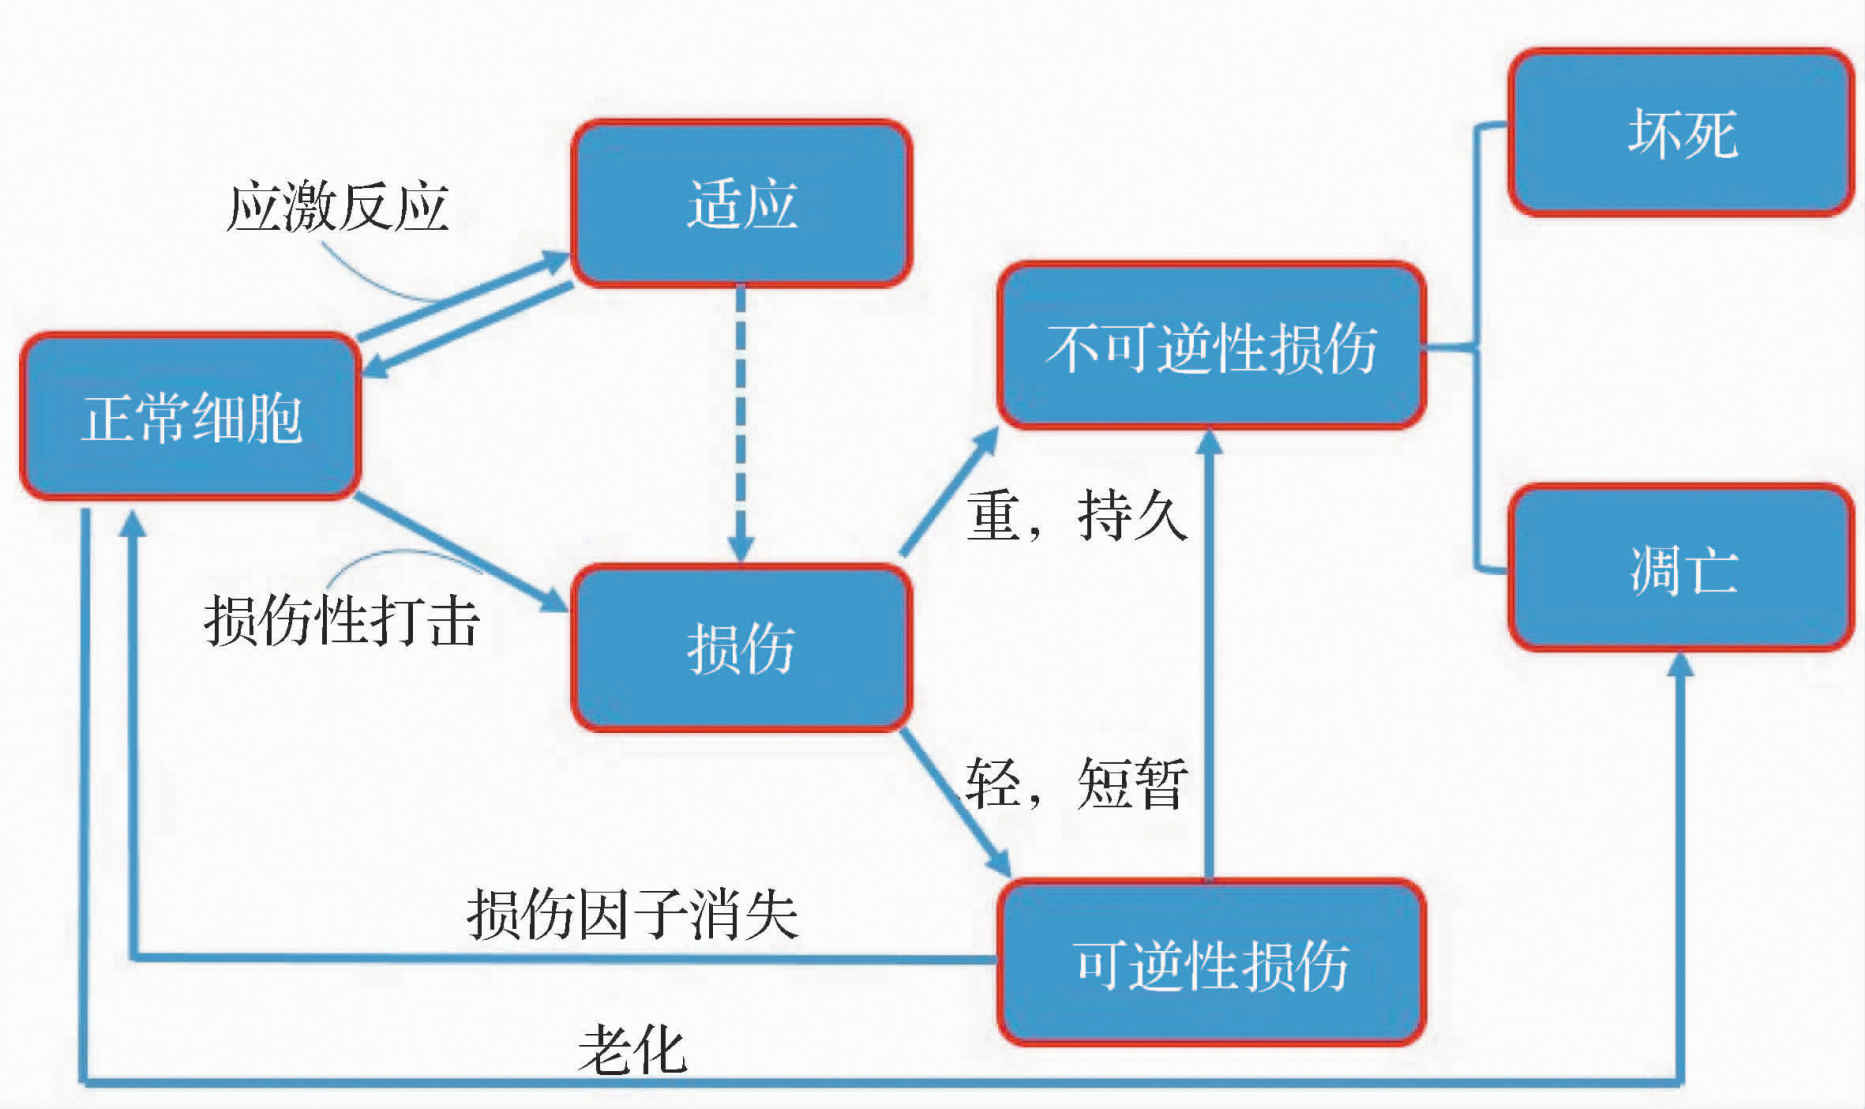
\includegraphics{./images/Image00023.jpg}
	\caption{组织细胞适应、损伤概览}
	\label{fig1-20}
\end{figure}

\section*{复习与思考}

{一、名词解释}

适应 萎缩 肠上皮化生 细胞水肿 脂肪变性 虎斑心 病理性钙化 凝固性坏死 干酪样坏死 液化性坏死 脑软化 坏疽 细胞凋亡

{二、问答题}

1. 机体组织细胞可出现哪几种适应性改变?

2. 久病卧床后肢体变细属于哪种类型的萎缩?为什么?

3. 试述肝脂变的原因和病变。

4. 何谓玻璃样变?好发于哪些部位?

5. 体内常见的色素有哪些?光镜下的特点是什么?

6. 试述坏死的镜下特点及结局。

7. 细胞的坏死和凋亡如何区别?

